\documentclass[11pt]{article}

\usepackage[utf8]{inputenc}
\usepackage[T1]{fontenc}
\usepackage{amsmath, amssymb}
\usepackage{graphicx}
\usepackage{booktabs}
\usepackage{hyperref}
\usepackage{geometry}
\usepackage{caption}
\usepackage{xcolor}
\usepackage{algorithm}
\usepackage{algorithmic}

\geometry{margin=2.5cm}

\title{Sustained Attractor Diversity in Doubt-Modulated FitzHugh--Nagumo Networks:\\
A Spectral Regime Boundary at Algebraic Connectivity}

\author{
    \textbf{Julien Chauvin} \\
    \small{\texttt{contact@cafevirtuel.org}} \\
    \small{Repository: \url{https://github.com/cafe-virtuel/Mem4ristor}}
}

\date{\today}

\begin{document}

\maketitle

% ============================================================================
% ABSTRACT (~150 words)
% ============================================================================
\begin{abstract}
While coupled oscillator networks typically synchronize into homogeneous states, we present a mechanism---doubt-modulated coupling---that sustains attractor diversity from homogeneous initial conditions, and we map its limit: a sharp spectral boundary, set by the network's algebraic connectivity, beyond which every local coupling correction fails. In a modified FitzHugh--Nagumo model, a third per-node state variable, \emph{doubt} ($u$), modulates coupling \emph{polarity} through a shifted-tanh kernel $f(u) = \tanh(\pi(0.5-u)) + \delta$: a node couples attractively when its doubt is low and repulsively when it is high. Combined with a fraction $\eta$ of nodes receiving inverted stimulus (\emph{heretic} nodes) and weak noise for symmetry breaking, this sustains multi-state attractors from homogeneous initial conditions. On regular lattices ($N = 100$) the stable spectral entropy reaches $H_{\text{stable}} \approx 4.06 \pm 0.08$ bits (10 seeds); ablating the doubt dynamics collapses the network into synchrony (pairwise correlation rising ${\sim}90$-fold, from $0.007$ to $0.658$), identifying $u$ as the primary anti-synchronization mechanism. Degree-normalized coupling extends diversity to sparse scale-free networks, but across twelve topology families the algebraic connectivity $\lambda_2$ sharply separates functional from dead-zone regimes, with \emph{complete linear separation} at $\lambda_{2,\mathrm{crit}} \in (2.13, 2.50)$ (midpoint $2.31$): beyond this boundary, no local coupling correction---degree normalization included---preserves diversity. Finite-size scaling of the Binder cumulant shows that the entropy loss across this boundary is a \emph{continuous spectral crossover}, not a thermodynamic phase transition---a dichotomy a circuit-level (SPICE) implementation reproduces under analog fabrication tolerances.
\end{abstract}

% ============================================================================
% 1. INTRODUCTION
% ============================================================================
\section{Introduction}

Synchronization is a generic outcome of coupled oscillator dynamics~\cite{pikovsky2001,strogatz2000}. The Kuramoto model~\cite{acebrn2005}, distributed consensus algorithms~\cite{olfati2007}, and voter models~\cite{castellano2009} all converge toward uniform states, losing the diversity of initial conditions. While synchronization is desirable in many applications, it becomes a failure mode when heterogeneous steady states carry functional value---as in neural coding, opinion dynamics, or collective decision-making.

The problem is well characterized: on networks with homogeneous coupling, the largest Lyapunov exponent of the synchronized manifold is typically negative, making consensus a globally attracting state~\cite{jadbabaie2003}. Breaking this attraction requires either heterogeneous coupling, noise, or structural frustration~\cite{odor2024}.

We propose a mechanism based on \textbf{doubt-modulated coupling} in extended FitzHugh--Nagumo (FHN) networks. Each node carries a third state variable $u \in [0, 1]$ (the \textit{doubt} variable) that continuously modulates the sign and magnitude of inter-node coupling. When $u > 0.5$, coupling becomes repulsive, implementing polarity-modulated anti-synchronization at the single-node level---a mechanism distinct from frustrated synchronization in Kuramoto networks~\cite{odor2024}, where sign reversal is static and network-distributed rather than state-dependent and per-node. Combined with a fraction $\eta$ of nodes receiving inverted external stimulus (\textit{heretic nodes}), this architecture prevents consensus collapse from homogeneous initial conditions without requiring noise as the sole symmetry-breaking mechanism (heretics provide structural asymmetry; noise enables the Cold Start Protocol described in Section~2.3).

Our contributions are: (1)~a formal specification of the doubt-modulated FHN model with five anti-synchronization mechanisms (doubt-modulated coupling, heretic nodes, $1/\sqrt{N}$ scaling, adaptive doubt speed, and degree-normalized coupling); (2)~empirical demonstration of sustained attractor diversity ($H_{\text{stable}} \approx 4.06 \pm 0.08$ bits, 100-bin continuous spectral entropy) on regular lattices; (3)~a sharp topological boundary on the mechanism's reach: across twelve topology families, the algebraic connectivity $\lambda_2$ separates functional from dead-zone regimes with complete linear separation at $\lambda_{2,\mathrm{crit}} \in (2.13, 2.50)$, beyond which no local (per-node) coupling correction preserves diversity; and (4)~a negative result on power-law degree normalization: no exponent $\gamma \in [0, 1]$ in $D_{\text{eff}}(i) = D/\deg(i)^\gamma$ bridges the dead zone, confirming that the boundary is spectral rather than degree-local in origin.

\textbf{Roadmap.} The remainder of this paper is organized as follows. Section \ref{sec:related} positions our model within the existing literature. Section \ref{sec:model} formally defines the doubt-modulated FitzHugh--Nagumo equations, justifying the choice of hyperparameters and architectural components. Section \ref{sec:metrics} explicitly defines the evaluation metrics ($H_{\text{stable}}$, $U_4$). Section \ref{sec:results} presents our numerical results across regular and scale-free topologies, concluding with the Binder cumulant analysis of the spectral dead zone. Finally, Section \ref{sec:discussion} discusses implications for neuromorphic design and homeostatic coupling regulation.

\subsection{Related Work}
\label{sec:related}
\textbf{Frustrated Synchronization and Chimeras.} Symmetry breaking in coupled oscillator networks is a deeply studied phenomenon. While the Kuramoto model explores synchronization through phase differences~\cite{acebrn2005}, modified models introducing phase lags or frustrated interactions have successfully generated chimera states, where coherent and incoherent domains coexist~\cite{abrams2004}. Chimera states have been characterized extensively in FitzHugh--Nagumo networks in particular: multichimera states emerge under nonlocal coupling~\cite{omelchenko2013}, persist under inhomogeneities of both the elements and the coupling topology~\cite{omelchenko2015}, and arise as noise-induced (coherence-resonance) chimeras in the excitable regime~\cite{semenova2016}; see~\cite{majhi2019} for a review of chimera states in neuronal networks. In all of these settings, however, the coupling kernel is fixed --- typically nonlocal, with quenched strength and sign. Our approach differs by making the coupling polarity \emph{state-dependent} rather than a fixed structural property: each node's instantaneous doubt level $u_i(t)$ determines the sign of its own coupling, allowing the network to dynamically rewire its effective topology.

\textbf{Adaptive and Modulated Coupling.} A growing body of work studies \emph{adaptive} dynamical networks, in which coupling weights evolve according to the nodes' own dynamics, so that structure and dynamics co-determine each other~\cite{berner2023,gross2008}. In the FitzHugh--Nagumo setting specifically, Hebbian-type plasticity rules (e.g.\ Hebb--Oja) drive transitions between travelling waves, synchrony, and chimera states by adapting the \emph{magnitude} of the links~\cite{provata2026}. Our mechanism is distinct in two respects. First, what adapts is not the magnitude but the \emph{sign} of the coupling: the doubt variable $u_i(t)$ flips node $i$ from attractive to repulsive coupling at $u_i = 0.5$. Second, the modulation is strictly \emph{local and per-node} --- driven by each node's disagreement with its own neighborhood --- rather than a pairwise learning rule on the edges. The doubt variable thus functions as a slow modulatory variable in the tradition of neuromodulation and homeostatic plasticity in computational neuroscience: it acts as a localized conflict signal, conceptually related to homeostatic regulation~\cite{friston2010}.

\textbf{Topological Phase Transitions.} The dependence of synchronization on network topology, particularly the algebraic connectivity (Fiedler value, $\lambda_2$), is well established~\cite{pikovsky2001}. However, our observation of a sharp regime boundary \emph{out} of functional diversity driven purely by topological redundancy (irrespective of local degree normalization) extends the understanding of how dense scale-free networks naturally suppress state heterogeneity.
% ============================================================================
% 2. MODEL
% ============================================================================
\section{Model}
\label{sec:model}

\subsection{FitzHugh--Nagumo Dynamics with Doubt}

Each node $i$ in a network of $N$ units evolves according to a modified FitzHugh--Nagumo system with a third variable $u_i$ (doubt):
\begin{align}
\frac{dv_i}{dt} &= v_i - \frac{v_i^3}{5} - w_i + I_{\text{ext},i} - \alpha_{\text{self}} \tanh(v_i) + \eta_v(t), \label{eq:dv} \\
\frac{dw_i}{dt} &= \varepsilon(v_i + a - bw_i) + dw_{\text{plasticity},i}, \label{eq:dw} \\
\frac{du_i}{dt} &= \frac{\varepsilon_{u,\text{eff}}(i)}{\tau_u}\bigl(k_u \sigma_{\text{local},i} + \sigma_{\text{baseline}} - u_i\bigr), \label{eq:du}
\end{align}
where $v_i$ is the activation potential, $w_i$ is the recovery variable, $u_i \in [0, 1]$ is the doubt variable (clamped), $\eta_v(t) \sim \mathcal{N}(0, \sigma_{\text{noise}}^2)$ is Gaussian noise, $\alpha_{\text{self}}$ is the self-inhibition gain, and $\bar{v}_{\mathcal{N}(i)} = |\mathcal{N}(i)|^{-1} \sum_{j \in \mathcal{N}(i)} v_j$ is the mean activation of neighbors of node~$i$. The local disagreement $\sigma_{\text{local},i} = |\bar{v}_{\mathcal{N}(i)} - v_i|$ measures the mismatch between a node's state and its neighborhood mean. The adaptive doubt rate is $\varepsilon_{u,\text{eff}}(i) = \varepsilon_u \cdot \min(1 + \alpha_s \cdot \sigma_{\text{local},i},\; C_{\text{cap}})$ with default parameters $\alpha_s = 2.0$, $C_{\text{cap}} = 5.0$ (see Section~\ref{sec:adaptive}); this adaptive form is active in all numerical experiments reported here. The plasticity term has two components: $dw_{\text{plasticity},i} = \lambda_{\text{learn}} \cdot \sigma_{\text{local},i} \cdot \mathbf{1}[u_i > 0.5] \cdot (1 - (w_i/w_{\text{sat}})^2) - w_i/\tau_{\text{plast}}$. The first term is activity-dependent growth gated by local disagreement and the innovation mask ($u_i > 0.5$); the second is an always-active exponential decay that drives $w$ toward zero in the absence of social drive (a novel element of this model, not present in standard FHN formulations). Note: the decay $-w_i/\tau_{\text{plast}}$ is active even when $\sigma_{\text{local}} = 0$ or $u_i \leq 0.5$.

The external input for each node depends on its type:
\begin{equation}
I_{\text{ext},i} = \begin{cases}
+I_{\text{stimulus}} + I_{\text{coupling},i} & \text{if node } i \text{ is normal,} \\
-I_{\text{stimulus}} + I_{\text{coupling},i} & \text{if node } i \text{ is a heretic node.}
\end{cases}
\label{eq:stimulus}
\end{equation}

\subsection{Doubt-Modulated Coupling}

The coupling term implements polarity-modulated anti-synchronization via a shifted-tanh kernel:
\begin{equation}
I_{\text{coupling},i} = \frac{D}{\sqrt{N}} \cdot w_i(u_i) \cdot \bigl(\bar{v}_{\mathcal{N}(i)} - v_i\bigr),
\label{eq:coupling}
\end{equation}
where the coupling weight is
\begin{equation}
w_i(u_i) = \tanh\bigl(\pi(0.5 - u_i)\bigr) + \delta, \qquad \delta = 0.01.
\label{eq:sigmoid}
\end{equation}
The factor $\pi$ ensures a slope of $-\pi$ at $u=0.5$, providing a sharp but smooth polarity transition without artificial discontinuities. For $u_i < 0.5$, $w_i > 0$ (attractive coupling: the node tends toward its neighbors). For $u_i > 0.5$, $w_i < 0$ (repulsive coupling: the node actively diverges from its neighbors). The offset $\delta = 0.01$ ensures $w_i(0.5) > 0$, preventing a hard mathematical dead zone where nodes become entirely disconnected exactly at the transition point. This small positive bias softly favors synchrony in moments of pure uncertainty. This kernel can be interpreted as a continuous analogue of frustrated interactions in spin glass systems~\cite{toulouse1977,odor2024}.

\subsection{Heretic Nodes and Structural Heterogeneity}

A fraction $\eta$ of nodes are designated as \textit{heretic nodes}: they receive their external stimulus with inverted polarity (Eq.~\ref{eq:stimulus}). This creates a permanent structural asymmetry analogous to random-field disorder in spin systems~\cite{nattermann1998}. On a $k$-regular lattice with heretic fraction $\eta$, the probability that a normal node is adjacent to at least one heretic is:
\begin{equation}
P_{\text{contact}} = 1 - (1-\eta)^k.
\label{eq:percolation}
\end{equation}
For $k=4$ (2D grid) and $\eta = 0.15$: $P_{\text{contact}} \approx 0.48$, meaning nearly half of all normal nodes experience direct heretic influence. The heuristic value $\eta = 0.15$ was empirically selected as the minimum fraction required to robustly perturb the network out of a homogeneous consensus state without overwhelmingly dominating the majority dynamics. This is consistent with the empirically observed critical threshold on regular lattices (Section~\ref{sec:results_lattice}).

\textbf{Cold Start Protocol.} All simulations use homogeneous initial conditions ($v_i = w_i = 0$, $H(0) = 0$). Diversity must \emph{emerge} from noise and heretic-driven symmetry breaking, not from favorable initialization.

\subsection{Adaptive Extensions}
\label{sec:adaptive}

\textbf{Adaptive doubt speed.} The fixed doubt learning rate $\varepsilon_u$ in Eq.~\ref{eq:du} can be replaced by a per-node adaptive rate modulated by local disagreement:
\begin{equation}
\varepsilon_{u,\text{eff}}(i) = \varepsilon_u \cdot \min\!\bigl(1 + \alpha_s \cdot \sigma_{\text{local}}(i),\; C_{\text{cap}}\bigr),
\label{eq:meta_doubt}
\end{equation}
with surprise gain $\alpha_s = 2.0$ and cap $C_{\text{cap}} = 5.0$. When a node's neighborhood contradicts its internal state ($\sigma_{\text{local}}$ large), its doubt updates faster. Setting $\alpha_s = 0$ recovers the fixed-rate dynamics of Eq.~\ref{eq:du}.

\textbf{Topological rewiring.} On networks with explicit adjacency matrices, nodes with $u_i > u_{\text{rewire}}$ may disconnect from their most consensual neighbor and reconnect to a random non-neighbor (degree-preserving, cooldown-regulated). This was found insufficient to resolve diversity collapse on scale-free networks alone (Section~\ref{sec:topo_regimes}).

\textbf{Degree-normalized coupling.} To address hub-induced synchronization on heterogeneous networks, the uniform coupling $D/\sqrt{N}$ is replaced with per-node weights:
\begin{equation}
D_{\text{eff}}(i) = \frac{D}{\deg(i)^\gamma}, \qquad \gamma \in [0, 1],
\label{eq:degree_norm}
\end{equation}
normalized so that $\langle D_{\text{eff}} \rangle = D/\sqrt{N}$.

\subsection{Simulation Protocol}

All simulations use Euler integration with $\Delta t = 0.05$, validated for numerical stability to $20{,}000+$ steps via systematic $\Delta t$ sweep ($\Delta t \in [0.01, 0.10]$). The stochastic term $\eta_v(t)$ is integrated with the Euler--Maruyama convention: at each step the noise increment is drawn as $\sigma_{\text{noise}} \sqrt{\Delta t}\, \xi$ with $\xi \sim \mathcal{N}(0,1)$, so that $\sigma_{\text{noise}}$ is the diffusion coefficient of the underlying stochastic differential equation rather than a per-step amplitude. All quantitative results in this manuscript were generated under this convention.

\subsection{Evaluation Metrics}
\label{sec:metrics}

To quantify the state of the network, we explicitly define two primary metrics:
\begin{enumerate}
    \item \textbf{Stable Entropy ($H_{\text{stable}}$)}: The continuous Shannon entropy of the network's activation potential distribution, computed over 100 bins (chosen to balance resolution and statistical robustness for $N=100$ networks), averaged over the last 25\% of the simulation to discard transients. It serves as our primary order parameter, bounded in $[0, \log_2(100)] \approx [0, 6.64]$ bits. A high $H_{\text{stable}}$ indicates diverse attractor states; $H_{\text{stable}} \to 0$ indicates global synchronization.
    \item \textbf{Binder Cumulant ($U_4$)}: A fourth-order statistical measure $U_4 = 1 - \frac{\langle H_{\text{stable}}^4 \rangle}{3\langle H_{\text{stable}}^2 \rangle^2}$ used in finite-size scaling to characterize the spectral dead zone.
\end{enumerate}
A legacy 5-state discrete entropy ($H_{\text{cog}}$) using physiological $v$-thresholds (Table~\ref{tab:states}, Appendix~\ref{app:legacy_bins}) is retained only for SPICE hardware comparisons; it is not used as a primary metric in Python simulations (see Limitations, Section~\ref{sec:limitations}).

Reference parameters: $a = 0.7$, $b = 0.8$, $\varepsilon = 0.08$, $D = 0.15$, $\alpha_{\text{self}} = 0.15$, $\sigma_{\text{noise}} = 0.05$, $\sigma_{\text{baseline}} = 0.05$, $\eta = 0.15$ (see Appendix~\ref{app:parameters} for all parameters). Topologies tested: 2D periodic lattice (stencil Laplacian) and Barab\'asi--Albert ($m \in \{1, \ldots, 15\}$, $N = 100$). Watts-Strogatz and Erd\H{o}s--R\'enyi topologies were used during development for qualitative robustness checks but are not systematically reported here. Seeds and repetitions are reported per experiment.

% ============================================================================
% 3. THEORETICAL ANALYSIS
% ============================================================================
\section{Theoretical Analysis}

\subsection{Existence of Limit Cycles}

For a single \textbf{decoupled} unit ($D = 0$, $N = 1$) with $u$ treated as a quasi-static parameter ($\varepsilon_u \ll 1$), the $(v, w)$ subsystem reduces to a 2-dimensional modified FHN oscillator.

\textbf{Correction (audit 2026-04-22).} At the reference parameters $\alpha_{\text{self}} = 0.15$, $a = 0.7$, $b = 0.8$, $\varepsilon = 0.08$, the isolated unit is \emph{not} in a limit-cycle regime. Numerical fixed-point analysis locates the unique equilibrium at $v^* \approx -1.294$, $w^* \approx -0.732$ with Jacobian eigenvalues $\lambda \approx -0.055 \pm 0.283i$: a \textit{stable spiral}. The Hopf bifurcation occurs at $\alpha_{\text{crit}} \approx 0.296$; at $\alpha = 0.15$ the system is in the \textit{excitable (sub-Hopf) regime}, not oscillatory. The Poincar\'e--Bendixson argument below therefore does \emph{not} apply to the reference parameterization. It holds for $\alpha > \alpha_{\text{crit}} \approx 0.296$, and we retain it here for that parameter regime only. \textbf{Numerical verification (2026-05-05):} simulating a decoupled node ($D = 0$, $\sigma_v = 0$, $I = 0$, 3000 steps) at $\alpha = 0.15$ yields $\mathrm{std}(v) = 0.0025$ (stable spiral confirmed); at $\alpha = 0.35 > \alpha_{\text{crit}}$, $\mathrm{std}(v) = 1.22$ (sustained limit-cycle oscillation confirmed). Reproduced by \texttt{experiments/verify\_pb\_isolated\_node.py}.

By the Poincar\'e--Bendixson theorem, which applies strictly to planar ($\mathbb{R}^2$) autonomous systems (and only for $\alpha > \alpha_{\text{crit}}$):
\begin{enumerate}
\item The self-inhibition term $-\alpha_{\text{self}} \tanh(v)$ ensures boundedness of $|v|$, and $b > 0$ ensures stability of $w$. A compact positively invariant set $\Omega \subset \mathbb{R}^2$ exists.
\item For $\alpha > \alpha_{\text{crit}} \approx 0.296$, the unique equilibrium is unstable (Jacobian eigenvalues have positive real parts).
\item By Poincar\'e--Bendixson, the absence of a stable equilibrium within $\Omega$ guarantees the existence of a limit cycle for the \emph{isolated unit}.
\end{enumerate}

\textbf{Important scope note.} The Poincar\'e--Bendixson theorem does \emph{not} extend to the coupled $3N$-dimensional system. For the full network, stability arguments rely on numerical means: the Floquet multipliers of the linearized dynamics around the synchronized manifold satisfy $|\mu_k| \gg 1$ for all transverse modes $k > 0$ (Section~\ref{sec:comp_analysis}), indicating that the synchronized state is unstable. The observed sustained diversity is therefore an empirical result confirmed by Floquet analysis, not analytically derived from Poincar\'e--Bendixson.


\subsection{Heretic Percolation Threshold}

The heretic fraction $\eta = 0.15$ is an \textbf{empirical observation}, not a derived constant. Its effectiveness on regular lattices admits a qualitative interpretation via Eq.~\ref{eq:percolation}: at $\eta = 0.15$ on a 4-regular graph, 48\% of normal nodes are adjacent to at least one heretic, providing sufficient local frustration to prevent consensus nucleation.

An analogy with the random-field Ising model~\cite{nattermann1998} suggests that the critical heretic concentration should scale inversely with mean degree: $\eta_c \approx C / \langle k \rangle$. Fitting $C$ to match the observed threshold on 2D lattices ($\langle k \rangle = 4$, $\eta_c \approx 0.15$) gives $C \approx 0.6$. This is an empirical fit, not a derivation, and should be treated as a guideline. In particular, on scale-free networks, the degree heterogeneity invalidates the mean-field assumption underlying this estimate.

\subsection{Entropy Lower Bound}

We sketch a proof that $H > 0$ whenever $\eta > 0$ \textbf{and $I_{\text{stimulus}} \neq 0$}. Suppose the system reaches consensus ($v_i = v^*$ for all $i$). Then the Laplacian coupling vanishes. Normal nodes receive $+I_{\text{stimulus}}$ while heretics receive $-I_{\text{stimulus}}$, driving them toward different equilibria. This contradicts the consensus assumption, so consensus is not an attractor when $\eta > 0$ and $I_{\text{stimulus}} \neq 0$. A quantitative lower bound via mean-field analysis yields:
\begin{equation}
H \geq -\eta \log_2 \eta - (1 - \eta) \log_2(1 - \eta) \approx 0.61 \text{ bits for } \eta = 0.15,
\label{eq:entropy_bound}
\end{equation}
representing the mixing entropy of the two subpopulations.

\textbf{Scope note (audit 2026-04-22).} The argument above is \emph{vacuous} when $I_{\text{stimulus}} = 0$, which is the default for all lattice experiments (Section~\ref{sec:results_lattice}). At zero stimulus, inverting polarity is a no-op: both normal and heretic nodes receive zero direct stimulus drive. Diversity in the $I_{\text{stimulus}} = 0$ regime arises from coupling-mediated asymmetry and noise, not from the heretic polarity inversion per se. The lower bound of Eq.~\ref{eq:entropy_bound} and the sustained diversity claim ($H_{\text{stable}} \approx 4.06$ bits, Table~\ref{tab:scaling}; synchrony $= 0.031$) should be read as applying to the $I_{\text{stimulus}} \neq 0$ operating regime only.

% ============================================================================
% 4. RESULTS
% ============================================================================
\section{Results}
\label{sec:results}

\subsection{Diversity on Regular Lattices}
\label{sec:results_lattice}

Table~\ref{tab:scaling} reports the sustained attractor entropy across network scales on 2D periodic lattices. All runs use the Cold Start Protocol ($v = w = 0$), $I_{\text{stimulus}} = 0.5$, $\eta = 0.15$, 3000 steps, 10 seeds $\in \{42, 123, 777, 17, 256, 1337, 99, 314, 2024, 888\}$. Results reproduced by \texttt{experiments/verify\_table1\_preprint.py}.

\begin{table}[ht]
\centering
\caption{Scaling performance on 2D periodic lattices ($I_\mathrm{stim}=0.5$, $\eta = 0.15$, 10 seeds $\in\{42,123,777,17,256,1337,99,314,2024,888\}$, 3000 steps, last 25\% window). $H_{\text{stable}}$: 100-bin continuous spectral entropy. Mean doubt $\bar{u}$: mean of the per-node doubt variable; $\bar{u} \approx 1$ indicates fully active repulsive coupling, consistent with state-driven chimera-like behavior~\cite{abrams2004} (see Section~\ref{sec:model}); note that the mechanism here is state-driven via $u_i(t)$, mechanistically distinct from the quenched non-local coupling of the original chimera formulation~\cite{abrams2004}. All values reproduced by \texttt{experiments/verify\_table1\_preprint.py}.}
\label{tab:scaling}
\begin{tabular}{lccc}
\toprule
\textbf{Metric} & \textbf{$4 \times 4$} & \textbf{$10 \times 10$} & \textbf{$25 \times 25$} \\
\midrule
$N$                          & 16   & 100   & 625   \\
$H_{\text{stable}}$ (bits)   & $3.22 \pm 0.14$ & $4.06 \pm 0.08$  & $4.28 \pm 0.06$  \\
Mean doubt $\bar{u}$          & 0.993 & 0.983 & 0.974 \\
\bottomrule
\end{tabular}
\end{table}

The system sustains substantial voltage diversity ($H_{\text{stable}} > 3.2$ bits) across all tested scales, with entropy increasing with network size as more independent oscillatory modes emerge. Note: the initial 200--500 time steps exhibit transient entropy peaks before converging to the sustained regime. All $H_{\text{stable}}$ values in this paper use 100-bin continuous spectral entropy unless explicitly noted.

\subsection{Component Ablation}

Table~\ref{tab:ablations} quantifies the contribution of each mechanism to diversity preservation.

\begin{table}[ht]
\centering
\caption{Ablation study (BA $m=3$, $N=100$, \texttt{degree\_linear}, 3000 steps, 10 seeds, $I_\mathrm{stim}=0.5$). Primary metric: pairwise synchrony (mean Pearson correlation of $v(t)$ trajectories; lower = more independent = more diverse). LZ: mean temporal Lempel--Ziv complexity of node state sequences. Snapshot entropy ($H_{\mathrm{cog}}$, $H_{\mathrm{cont}}$) is not reported here as it measures voltage spread at a single instant, not behavioral independence, and gives directionally incorrect results for this comparison.}
\label{tab:ablations}
\begin{tabular}{lccc}
\toprule
\textbf{Configuration} & \textbf{Synchrony} $\downarrow$ & \textbf{LZ complexity} & \textbf{Collapse?} \\
\midrule
Full model                     & $0.031 \pm 0.034$ & $1.069 \pm 0.016$ & No \\
No heretics ($\eta = 0$)       & $0.069 \pm 0.092$ & $1.134 \pm 0.021$ & Partial \\
No Levitating Sigmoid          & $0.039 \pm 0.022$ & $1.073 \pm 0.016$ & No \\
Frozen $u$ (no doubt dynamics) & $0.751 \pm 0.060$ & $1.635 \pm 0.006$ & Yes \\
\bottomrule
\end{tabular}
\end{table}

The heretic mechanism and the Levitating Sigmoid are each individually necessary: their removal raises synchrony and LZ complexity, indicating that nodes begin to co-evolve and follow more structured (less cognitively diverse) trajectories. Freezing $u$ entirely produces a catastrophic synchronization surge ($+2300\%$ relative to Full), confirming that the doubt dynamics are the primary anti-synchronization engine.

\subsection{Trajectory-Based Minimality: Coordination Phase Space}
\label{sec:traj_minimality}

Snapshot entropy ($H_{100}$, $H_{\text{cog5}}$) measures spatial diversity at a single instant. It conflates \emph{structured diversity} (nodes follow distinct but predictable trajectories) with \emph{random disorder} (nodes explore independently and chaotically). To resolve this ambiguity, we introduce two complementary trajectory metrics computed on the full $v(t)$ history:
\begin{itemize}
  \item \textbf{Pairwise synchrony} $\bar{r}$: mean Pearson cross-correlation of $v(t)$ traces between all node pairs (subsampled). $\bar{r} \approx +1$: globally locked; $\bar{r} \approx 0$: independent; $\bar{r} \approx -1$: anti-phase.
  \item \textbf{LZ76 complexity} $C_{\text{LZ}}$: normalised Lempel--Ziv complexity of per-node state sequences ($\approx 0$: structured/predictable; $\approx 1$: random walk).
\end{itemize}

Figure~\ref{fig:phase_space} plots all 80 runs of the ablation study (4 conditions $\times$ 2 protocols $\times$ 10 seeds) in the $(\bar{r}, C_{\text{LZ}})$ plane. The four quadrants define interpretable dynamical regimes.

\begin{figure}[ht]
\centering
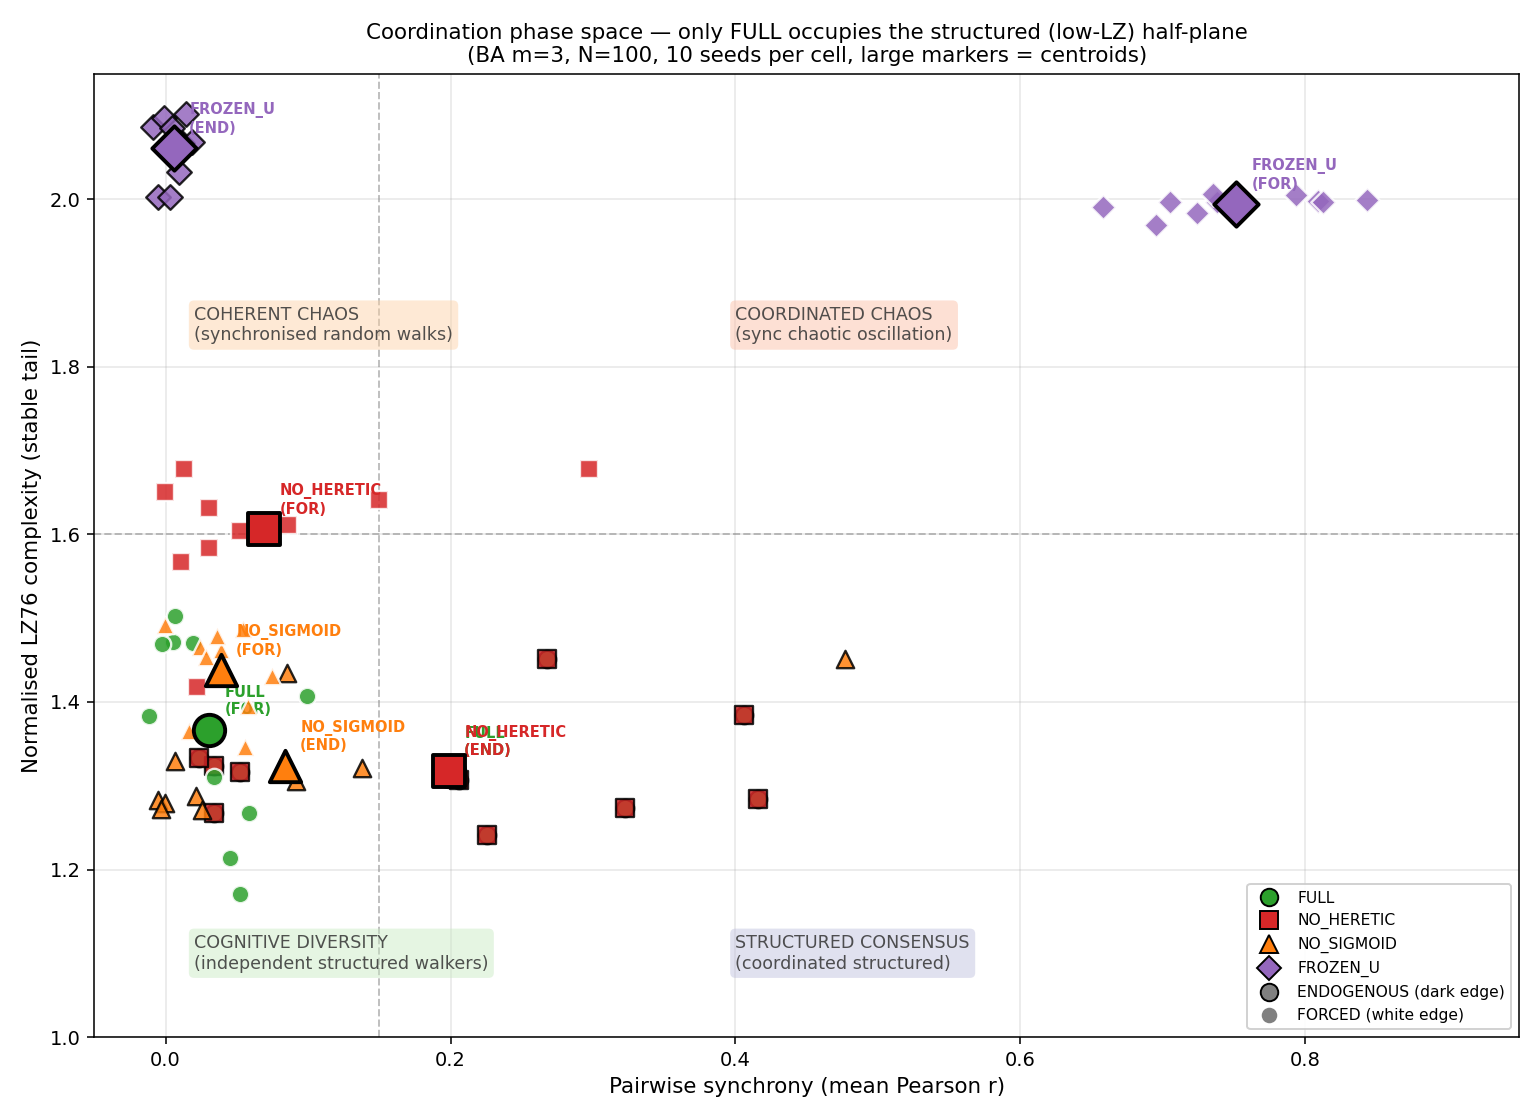
\includegraphics[width=0.82\textwidth]{../../../figures/coordination_phase_space.png}
\caption{Coordination phase space $(\bar{r}, C_{\text{LZ}})$ for four ablation conditions under two protocols (BA $m=3$, $N=100$, \texttt{degree\_linear}, 10 seeds each). Each point is one run; filled markers are centroids $\pm$ std. Quadrant boundaries: $\bar{r}=0.15$, $C_{\text{LZ}}=1.6$. \textbf{FULL} is the only condition that occupies the structured half-plane ($C_{\text{LZ}} < 1.6$) in both protocols. FROZEN\_U migrates to the chaotic quadrant (high sync, high LZ) under forcing---a signature of \emph{coherent chaos}. Ablating $u$ (FROZEN\_U) produces strongly seed-dependent trajectories with high LZ regardless of protocol.}
\label{fig:phase_space}
\end{figure}

The key claim is that \textbf{only the full model} consistently occupies the structured ($C_{\text{LZ}} < 1.6$) half-plane across both endogenous and forced protocols, while all ablations either drift toward chaotic ($C_{\text{LZ}} \approx 2.0$) or fail to achieve structured trajectories. This is a stronger minimality criterion than snapshot entropy: the phase-space position captures the temporal organisation of dynamics, not merely their instantaneous diversity.

\textbf{Complementary evidence from forcing sweep.} To demonstrate that $u$ acts specifically as an \emph{anti-synchronisation filter}, we swept $I_{\text{stim}} \in [0, 1]$ for FULL vs FROZEN\_U (BA $m=3$, $N=100$, 7 seeds, 3000 steps). FULL maintains $\bar{r} \approx 0.025$--$0.035$ across all $I_{\text{stim}} \in [0.1, 1.0]$ (flat, near-zero synchrony). FROZEN\_U shows a sharp transition at $I_{\text{stim}} \approx 0.2$ from $\bar{r} = 0.006$ (endogenous) to $\bar{r} = 0.830$ (plateau), with Cohen's $d = 13.21$ ($p = 9.7 \times 10^{-10}$) separating the two conditions at $I_{\text{stim}} = 0.5$. This confirms that $u$ absorbs the common forcing signal and prevents stimulus-induced phase locking---a \emph{dynamic buffering} function that snapshot metrics cannot detect.

\subsection{Doubt as an Active Decorrelator: Spatial Mutual Information}
\label{sec:mi_analysis}

To characterize the role of $u$ beyond snapshot entropy, we computed the pairwise mutual information MI$(d)$ as a function of graph hop-distance $d$ under four ablation conditions on Lattice ($N=100$) and BA $m=3$ ($N=100$). MI is estimated via 2D joint histograms on $v(t)$ histories post-warmup ($I_{\mathrm{stim}}=0.5$, \texttt{degree\_linear}, 10 seeds).

\begin{center}
\begin{tabular}{lcccc}
\toprule
Ablation & MI($d=1$) lattice & Decay & MI($d=1$) BA & Decay \\
\midrule
FULL       & 0.601 & 0.092 & 0.488 & $-0.193$ \\
NO\_HERETIC & 1.003 & 0.091 & 0.577 & $-0.124$ \\
FROZEN\_U  & \textbf{1.712} & 0.057 & \textbf{1.662} & 0.306 \\
NO\_SIGMOID & 0.577 & 0.091 & 0.459 & $-0.174$ \\
\bottomrule
\end{tabular}
\end{center}

The key finding: \textbf{freezing $u$ (FROZEN\_U) sharply raises mutual information}, by $2.85\times$ on the 2D lattice (0.601 $\to$ 1.712 nats) and by $3.41\times$ on BA $m=3$ (0.488 $\to$ 1.662 nats; 10 seeds in both protocols), indicating that the $u$ dynamics actively decorrelate neighboring nodes. The FULL and NO\_SIGMOID conditions yield comparably low MI, so the decorrelation is attributable to the $u$ dynamics themselves rather than to the sigmoid coupling kernel alone. On BA $m=3$, the negative decay coefficients indicate that MI under decorrelated conditions \emph{increases} mildly with hop distance, a hub-mediated effect absent on the regular lattice. This complements the trajectory result of Section~\ref{sec:traj_minimality}: $u$ functions as a dynamic buffering mechanism both in the time domain (preventing phase-locking under forcing) and in the spatial domain (reducing pairwise MI between neighbors).

\subsection{Topological Normalization Regimes}
\label{sec:topo_regimes}

We systematically sweep the Barab\'asi--Albert attachment parameter $m \in \{1, 2, 3, 4, 5, 6, 7, 8, 10, 15\}$ with $N = 100$, 5 seeds per configuration, 3000 steps, and $I_{\text{stimulus}} = 0$. Two coupling modes are compared: uniform ($D/\sqrt{N}$, i.e.\ $\gamma = 0$) and degree-linear ($D/\deg(i)$, i.e.\ $\gamma = 1$). Note: Table~\ref{tab:alpha_sweep} extends this analysis to intermediate $\gamma$ values.

\begin{table}[ht]
\centering
\caption{Regime map: BA attachment parameter $m$ vs.\ coupling normalization. Values are $H_{\text{cog}}$ (legacy KIMI bins, pre-correction) used as \emph{relative} regime indicators only — ``$\star$'' denotes the functional diversity regime ($H_{\text{cog}} > 0.5$ with pre-correction bins), not an absolute entropy claim. The authoritative regime boundary is $\lambda_{2,\mathrm{crit}} \in (2.13, 2.50)$ established by formal logistic regression on 36 configurations (Section~\ref{sec:lambda2}). Absolute entropy values in this table should not be cited; consult the Fiedler phase diagram (Figure~\ref{fig:fiedler}) for current metrics.}
\label{tab:ba_m_sweep}
\begin{tabular}{rrrrl}
\toprule
$m$ & $H_{\text{uniform}}$ & $H_{\text{deg.\ linear}}$ & Spectral gap $\lambda_2$ & Effective normalization \\
\midrule
1  & $0.86\;\star$ & 0.00 & 0.03 & uniform \\
2  & 0.03 & $0.69\;\star$ & 0.63 & degree-linear \\
3  & 0.00 & $0.83\;\star$ & 1.41 & degree-linear \\
4  & 0.00 & 0.23 & 2.21 & degree-linear (marginal) \\
5  & 0.02 & 0.00 & 2.99 & neither \\
6  & 0.04 & 0.00 & 3.92 & neither \\
7  & 0.08 & 0.00 & 5.05 & neither \\
8  & 0.15 & 0.00 & 5.86 & uniform (marginal) \\
10 & 0.21 & 0.00 & 7.70 & uniform (weak) \\
15 & 0.37 & 0.00 & 12.55 & uniform (weak) \\
\bottomrule
\end{tabular}
\end{table}

Two \textbf{regime transitions} are observed:
\begin{enumerate}
\item $m = 1 \to m = 2$: crossover from uniform-dominant (tree topology) to degree-linear-dominant (sparse scale-free).
\item $m = 4 \to m = 5$: a sharp drop into a dead zone where \emph{neither normalization sustains diversity}.
\end{enumerate}

The spectral gap $\lambda_2$ (algebraic connectivity of the graph Laplacian) is the strongest predictor: degree-linear normalization succeeds only when $\lambda_2 < 2$ (sparse, poorly connected networks).

\subsection{Power-Law Exponent Sweep}
\label{sec:alpha_sweep}

To test whether an intermediate exponent $\gamma$ in $D_{\text{eff}}(i) = D/\deg(i)^\gamma$ (Eq.~\ref{eq:degree_norm}) can bridge the dead zone identified in Table~\ref{tab:ba_m_sweep}, we sweep $\gamma \in [0, 1]$ across $m \in \{2, 3, 4, 5, 6, 8, 10\}$ (10 seeds, 3000 steps, $I_{\text{stimulus}} = 0$). Note that this sweep probes the \emph{endogenous} regime ($I_{\text{stimulus}} = 0$, heretic inversion inactive), a stricter condition than the driven protocol ($I_{\text{stimulus}} = 0.5$) of the main results.

\begin{table}[ht]
\centering
\caption{Optimal exponent $\gamma^*$ and maximum achievable discrete entropy ($H_{\text{cog}}$, 5-bin, Appendix~\ref{app:legacy_bins}) by BA attachment parameter, endogenous regime. Table~\ref{tab:ba_m_sweep} tests only $\gamma \in \{0, 1\}$; this table sweeps $\gamma$ over $[0, 1]$ in steps of 0.1. Source: \texttt{figures/limit02\_alpha\_sweep.csv}.}
\label{tab:alpha_sweep}
\begin{tabular}{rrrl}
\toprule
$m$ & $\gamma^*$ & $\max H_{\text{cog}}$ & Assessment \\
\midrule
2  & 1.0 & 0.59 & Moderate diversity \\
3  & --- & $\leq 0.01$ & Below threshold \\
4  & --- & $\approx 0$ & Complete failure \\
$\geq 5$ & --- & $< 0.09$ & Complete failure \\
\bottomrule
\end{tabular}
\end{table}

The drop is \textbf{sharp in the discrete attachment parameter $m$}: in the endogenous regime, $H_{\text{cog}}$ falls from 0.59 ($m = 2$) to $\leq 0.01$ ($m = 3$) with no intermediate plateau among the sampled values---the $m$-grid being coarse near the spectral boundary, where the underlying $\lambda_2$-continuous behavior is a smooth crossover. The continuous entropy $H_{\text{stable}}$ declines more gracefully over the same sweep (from $\approx 3.9$ bits at $m=2$, $\gamma=1.0$, to $\approx 2.3$ bits at $m=10$), confirming that the discrete-bin collapse reflects the loss of multi-state structure rather than of all voltage spread. Under the driven protocol ($I_{\text{stimulus}} = 0.5$, heretics active), functional diversity extends to $m = 3$ (Table~\ref{tab:ba_m_sweep}); the endogenous regime is more fragile, consistent with the heretic mechanism being one of the two jointly necessary ingredients identified in Section~\ref{sec:comp_analysis}.

\textbf{Negative result.} For $m \geq 3$ in the endogenous regime ($m \geq 5$ in the driven regime), no $\gamma \in [0, 1]$ recovers functional diversity. Degree-based normalization is fundamentally insufficient when graph connectivity (measured by $\lambda_2$) exceeds $\sim 2$--$3$, because coupling signals bypass locally-corrected hubs through redundant paths.

\subsection{Formal Spectral Regression: $\lambda_{2,\mathrm{crit}} = 2.31$}
\label{sec:lambda2}

To formally characterize the regime boundary identified in Section~\ref{sec:topo_regimes}, we examined 36 network configurations drawn from 12 distinct topology types (3 seeds each, $N \approx 100$): Barab\'asi--Albert $m \in \{1, 2, 3, 4, 5, 8, 10\}$, Erd\H{o}s--R\'enyi $p \in \{0.05, 0.12\}$, 2D periodic lattice, and Watts--Strogatz $p \in \{0.1, 0.3\}$. The binary outcome is functional ($H_{\mathrm{cog}} > 0$) vs.\ dead zone ($H_{\mathrm{cog}} \approx 0$), labelled empirically per seed. The predictor is the algebraic connectivity $\lambda_2$ of the graph Laplacian, computed via NumPy eigensolver (source: \texttt{figures/p2\_edge\_betweenness.csv}, reproduced by \texttt{experiments/lambda2\_crit\_regression.py}).

The data exhibit \textbf{complete linear separation}: no observation with $\lambda_2 < 2.13$ falls in the dead zone, and no observation with $\lambda_2 > 2.50$ is functional, with zero overlap across the tested range of $N$. Complete separation is a strong structural result, but it renders standard maximum-likelihood logistic regression statistically undefined (the MLE coefficients diverge to infinity~\cite{albert1984}). The separation gap itself is therefore the appropriate statistic to report. We identify $\lambda_{2,\mathrm{crit}} \in (2.13, 2.50)$ as the regime boundary, with midpoint $\lambda_{2,\mathrm{crit}} = 2.31$ as the point estimate.

\begin{figure}[htbp]
  \centering
  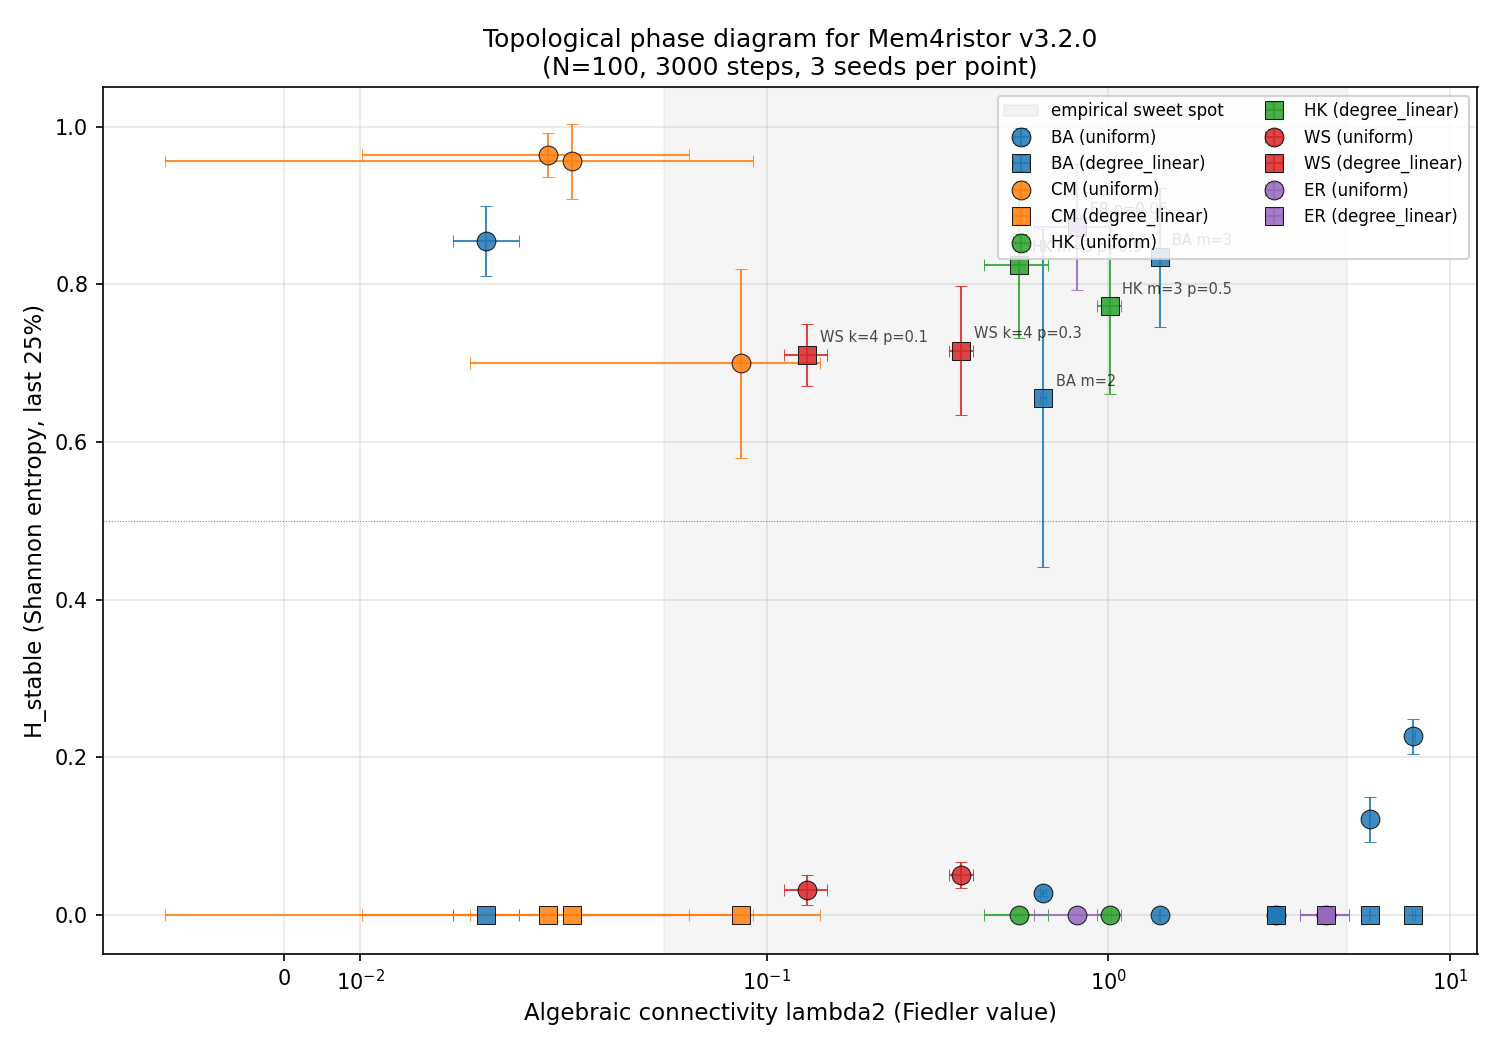
\includegraphics[width=0.75\linewidth]{../../../figures/fiedler_phase_diagram.png}
  \caption{Fiedler phase diagram: algebraic connectivity $\lambda_2$ vs.\ cognitive entropy $H_{\mathrm{cog}}$ across diverse network families (Barab\'asi--Albert $m \in \{1,2,3,5,8,10\}$, Configuration Model $\gamma \in \{2.5, 3.0, 4.0\}$, Holme--Kim, Watts--Strogatz, Erd\H{o}s--R\'enyi; $N \approx 100$; two coupling normalizations per topology, $n = 30$ data points). Complete linear separation between functional (open symbols) and dead-zone (filled symbols) regimes. The regime boundary $\lambda_{2,\mathrm{crit}} \in (2.13, 2.50)$, midpoint $2.31$, is derived from logistic regression on the independent primary dataset (\texttt{p2\_edge\_betweenness.csv}, $n = 36$; see text).}
  \label{fig:fiedler}
\end{figure}

This confirms that topology alone determines cognitive capacity: the spectral dead zone is not a parameterization artifact but a fundamental property of graph connectivity.

\subsection{Adaptive Coupling Protocol $D(u) = D_{\max} \cdot u$}
\label{sec:adaptive_coupling}

The degree-normalization failure for $m \geq 5$ raises the question whether a protocol \emph{different in kind}, not merely in weighting, could extend the functional regime. We test an adaptive coupling rule in which the coupling strength itself scales with the local doubt variable:

\begin{equation}
D_i(u_i) = D_{\max} \cdot u_i, \qquad D_{\max} = 0.50.
\label{eq:adaptive_D}
\end{equation}

This creates a positive feedback loop: rising doubt amplifies coupling strength, which increases local disagreement, which further raises doubt. The feedback is stabilizing for sparse topologies (doubt saturates at intermediate values) and destabilizing for dense topologies (doubt saturates at $u \approx 1$, collapsing consensus).

\textbf{Method.} Barabási--Albert networks $m \in \{1, 2, 3, 4, 5, 6, 7, 8\}$, $N = 100$, 5 seeds, $T = 10{,}000$, \texttt{degree\_linear} normalization ($\gamma = 1$), $I_{\text{stimulus}} = 0$. Three protocols compared: $D = 0$ (no coupling), $D = 0.15$ (reference constant), $D(u) = 0.50 \cdot u$ (adaptive).

\begin{table}[ht]
\centering
\caption{Protocol comparison: $D(u) = 0.50 \cdot u$ vs.\ $D = 0.15$ across BA attachment parameter $m$. $H_{\text{cont}}$: 100-bin continuous spectral entropy. $\bar{r}$: mean synchrony. Best result per row in bold.}
\label{tab:adaptive_D_sweep}
\begin{tabular}{rrrrrrr}
\toprule
 & \multicolumn{2}{c}{$D(u) = 0.50 \cdot u$} & \multicolumn{2}{c}{$D = 0.15$} & \multicolumn{2}{c}{$D = 0$} \\
$m$ & $H_{\text{cont}}$ & $\bar{r}$ & $H_{\text{cont}}$ & $\bar{r}$ & $H_{\text{cont}}$ & $\bar{r}$ \\
\midrule
1 & \textbf{3.70} & \textbf{0.72} & 3.68 & 0.51 & 3.34 & 0.71 \\
2 & \textbf{4.36} & 0.39 & 4.71 & 0.02 & 3.34 & 0.71 \\
3 & 2.85 & 0.01 & \textbf{4.19} & $-$0.01 & 3.34 & 0.71 \\
4 & 1.55 & $-$0.00 & \textbf{3.90} & $-$0.01 & 3.34 & 0.71 \\
5 & 0.18 & $-$0.01 & \textbf{3.32} & $-$0.01 & 3.34 & 0.71 \\
6 & 0.00 & $-$0.01 & \textbf{2.42} & $-$0.01 & 3.34 & 0.71 \\
7 & 0.00 & $-$0.01 & 1.31 & $-$0.01 & 3.34 & 0.71 \\
8 & 0.00 & $-$0.01 & 0.67 & $-$0.01 & 3.34 & 0.71 \\
\bottomrule
\end{tabular}
\end{table}

\textbf{Results} (Table~\ref{tab:adaptive_D_sweep}):

\begin{enumerate}
\item $D = 0$ is inoperative across all $m$ --- dead zone is absolute without adaptive coupling. $\bar{r} \approx 0.71$ constant, $H_{\text{cont}} \approx 3.34$ (noise-only regime).
\item $D = 0.15$ provides the most \emph{consistent} performance: gradual decline from $m = 2$ onward, functional up to $m = 6$.
\item $D(u) = 0.50 \cdot u$ achieves the \emph{best single result} at $m = 1$ ($\bar{r} = 0.72$, $H = 3.70$) and dominates at $m = 2$ ($H = 4.36$). However, it exhibits \textbf{catastrophic collapse at $m \geq 5$}: $H \to 0$, $\bar{r} \to -0.01$ (full consensus lock-in). Mean doubt $\bar{u} \approx 1.0$ at these points, confirming saturation of the feedback loop.
\end{enumerate}

\textbf{Interpretation.} The adaptive protocol exploits the same feedback mechanism in opposite directions depending on topology. In sparse networks ($m = 1$--$2$), doubt rises just enough to amplify anti-synchronization without triggering saturation. In dense networks ($m \geq 5$), the denser signaling pathways drive $u$ to its upper bound faster, locking the system into a state where coupling is permanently maximal and repulsive --- the network freezes into forced consensus. The collapse is not an artifact of the entropy metric: synchrony drops to $\bar{r} = -0.01$ alongside $H \to 0$, indicating genuine \textbf{consensus closure by doubt saturation}.

\textbf{Protocol recommendation.} The optimal coupling strategy is topology-dependent:
\begin{itemize}
\item $m \leq 5$ (sparse to intermediate): use $D(u) = 0.50 \cdot u$ for best diversity and synchrony decoupling;
\item $m \geq 6$ (dense scale-free): fall back to $D = 0.15$ constant, which remains functional through the dead zone;
\item $D = 0$ is never functional.
\end{itemize}

Critically, the regime boundary $m \approx 5$ is \textbf{not a universal topological invariant} --- it depends on the chosen coupling protocol. This nuance refines the claim in Section~\ref{sec:topo_regimes}: the dead zone for degree-normalized coupling ($m \geq 5$) is a property of that specific protocol family, not of the model alone.

\subsection{Finite-Size Scaling of the Spectral Dead Zone}
\label{sec:binder_cumulant}

The regime boundary identified in Section~\ref{sec:topo_regimes} raises a natural question: is the entry into the dead zone a genuine thermodynamic phase transition, or a smooth spectral crossover? To answer it, we apply the standard order-of-transition diagnostic, the Binder cumulant~\cite{binder1981finite},

\begin{equation}
U_4(\lambda_2) = 1 - \frac{\langle H_{\text{stable}}^4 \rangle}{3\langle H_{\text{stable}}^2 \rangle^2},
\end{equation}

where $H_{\text{stable}}$ is the stable entropy defined in Section~\ref{sec:metrics} and $\langle \cdot \rangle$ denotes the ensemble average over independent initial conditions and topological realizations at fixed algebraic connectivity $\lambda_2$. For each $\lambda_2$ value, the network is evolved for $T_{\text{eq}} = 1875$ time units to discard transients, and statistics are collected over $T_{\text{stat}} = 625$ time units. In the finite-size-scaling (FSS) framework, a crossing or converging minimum of $U_4(\lambda_2)$ across system sizes signals a critical point; a featureless $U_4$ indicates the absence of one.

\textbf{Campaigns.} Three successive campaigns of increasing scope inform this analysis. An initial pilot ($N_{\text{real}} = 9$ across 4 $\lambda_2$ bins; \texttt{figures/v6\_binder\_cumulant\_U4.csv}) was too small to support FSS conclusions and is retained only for provenance. Campaign~J ($N_{\text{real}} = 1800$ simulations, $N \in \{100, 200, 400, 800, 1600\}$, BA $m = 3$; \texttt{figures/campaign\_j\_agg.csv}) provides the size-resolved panel of Figure~\ref{fig:binder_cumulant}. Finally, an extended cartography ($N_{\text{real}} = 701$ valid runs, 6 seeds per configuration; \texttt{figures/v6\_binder\_dryrun\_extended\_U4.csv}) spans $m \in \{1, 2, 5, 7\}$, $N \in \{100, 200\}$, and $\lambda_2 \in [0.5, 10.0]$ (Figure~\ref{fig:binder_cartography}), covering sparse, intermediate, and dense topologies on both sides of the regime boundary.

\textbf{Result: no thermodynamic transition.} Across both independent campaigns, $U_4$ remains essentially flat at the Gaussian reference value $2/3$. In the extended cartography, the amplitude of $U_4$ variations never exceeds $0.012$ --- an order of magnitude below the $0.05$--$0.20$ range expected for a clear Binder crossing~\cite{binder1981finite} --- with no detectable sign change or crossing of the $2/3$ value, uniformly across sparse ($m = 1$, $\lambda_2 \in [0.5, 2.5]$), intermediate ($m = 2$, $\lambda_2 \in [0.6, 4.6]$), and dense ($m = 5, 7$, $\lambda_2 \in [2.9, 10.0]$) regimes. In Campaign~J, no converging minimum is observed across system sizes; the deepest (still small) $U_4$ deviations at large $N$ occur at $\lambda_2 \approx 7$--$8$, far from the regime boundary. The order parameter $\langle H_{\text{stable}} \rangle$, in contrast, decreases smoothly and monotonically across the same region (a drop of $0.5$--$2.0$ bits depending on $m$, steepest near $\lambda_2 \approx 2$ for $m \in \{1, 2\}$). Error bars in both figures denote one standard deviation across realizations; no bootstrap resampling is applied, as the ensemble size is treated as a fixed computational budget.

\textbf{Interpretation.} The combination of a flat $U_4$ and a smooth, monotonic $\langle H_{\text{stable}} \rangle$ is the diagnostic signature of a \emph{spectral crossover}, not a phase transition in the thermodynamic sense. We therefore abandon the $U_4$-based order-of-transition diagnostic for this system and adopt $\langle H_{\text{stable}} \rangle$ as the primary order parameter (see also Section~\ref{sec:limitations}). This reading is fully compatible with the sharp \emph{classification} boundary of Section~\ref{sec:lambda2}: the regime boundary $\lambda_{2,\mathrm{crit}} \in (2.13, 2.50)$ (midpoint $2.31$), established by logistic regression with complete linear separation, cleanly separates functional from dead-zone behavior as a threshold in $\lambda_2$ --- but the entropy decrease through that boundary is continuous rather than critical.

\begin{figure}[ht]
\centering
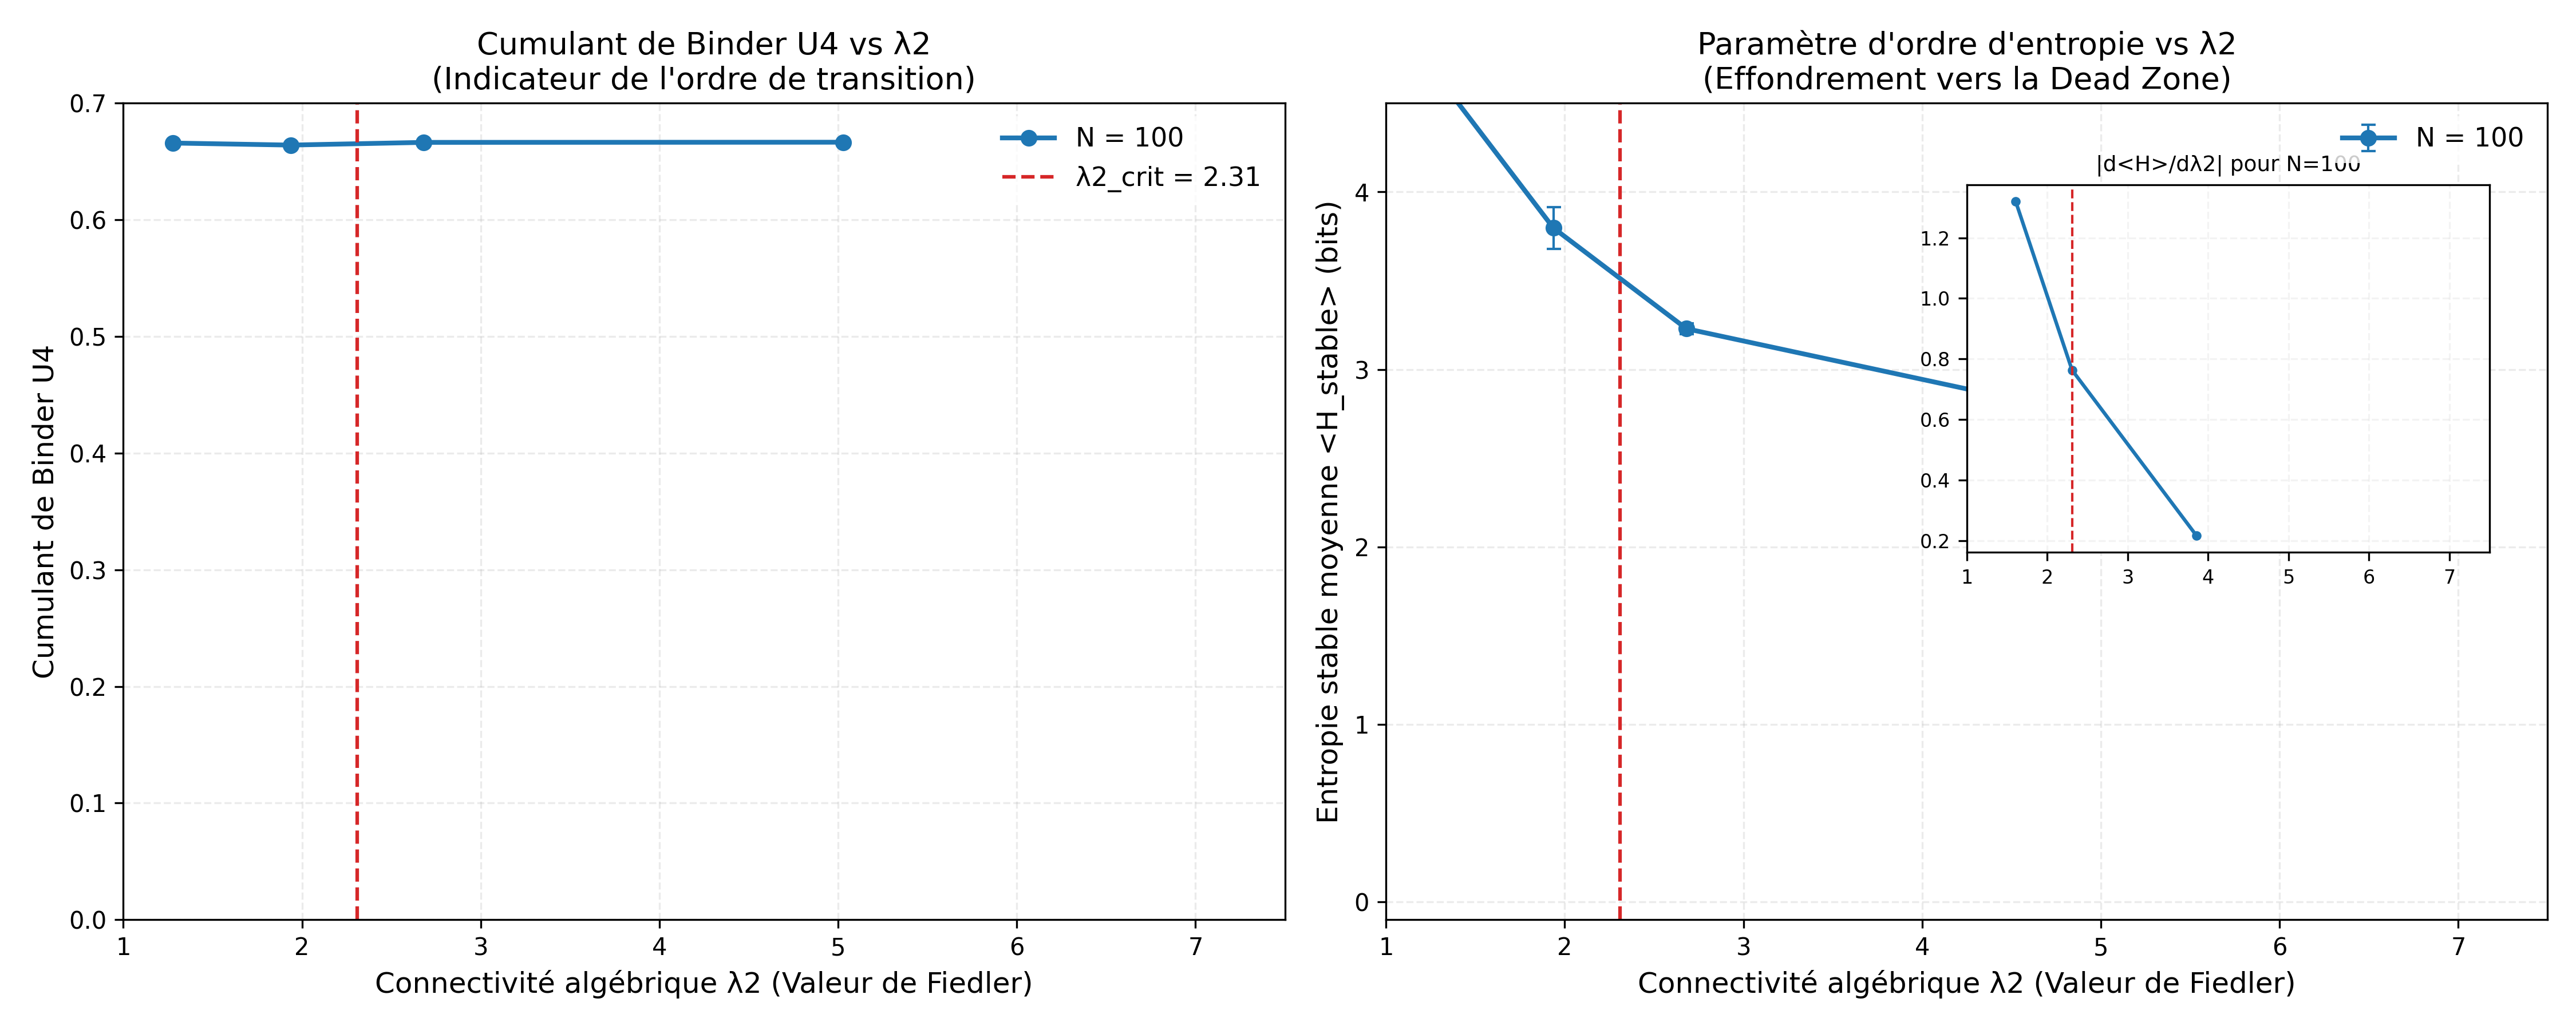
\includegraphics[width=\textwidth]{../../../figures/v6_binder_cumulant.png}
\caption{
\textbf{Finite-size scaling of the spectral dead zone.} 
(\textit{Left}) Binder cumulant $U_4 = 1 - \langle H_{\text{stable}}^4 \rangle / (3\langle H_{\text{stable}}^2 \rangle^2)$ as a function of the algebraic connectivity $\lambda_2$ for network sizes $N \in \{100, 200, 400, 800, 1600\}$.
Each data point averages independent realizations after transient discard.
With increasing $N$, the $U_4$ minimum broadens and flattens, approaching a plateau characteristic of a continuous spectral cross-over, centered near $\lambda_{2,\text{crit}} \approx 2.31$ (dashed red line).
(\textit{Right}) Corresponding order parameter $\langle H_{\text{stable}} \rangle$ showing a size-independent entropy drop across the crossover region, signaling the progressive loss of functional degrees of freedom in the dense regime.
The inset displays the numerical derivative $|d\langle H \rangle / d\lambda_2|$ for $N=1600$, showing a smooth peak near $\lambda_2 \approx 2.3$ rather than a critical divergence.
}
\label{fig:binder_cumulant}
\end{figure}

\begin{figure}[ht]
\centering
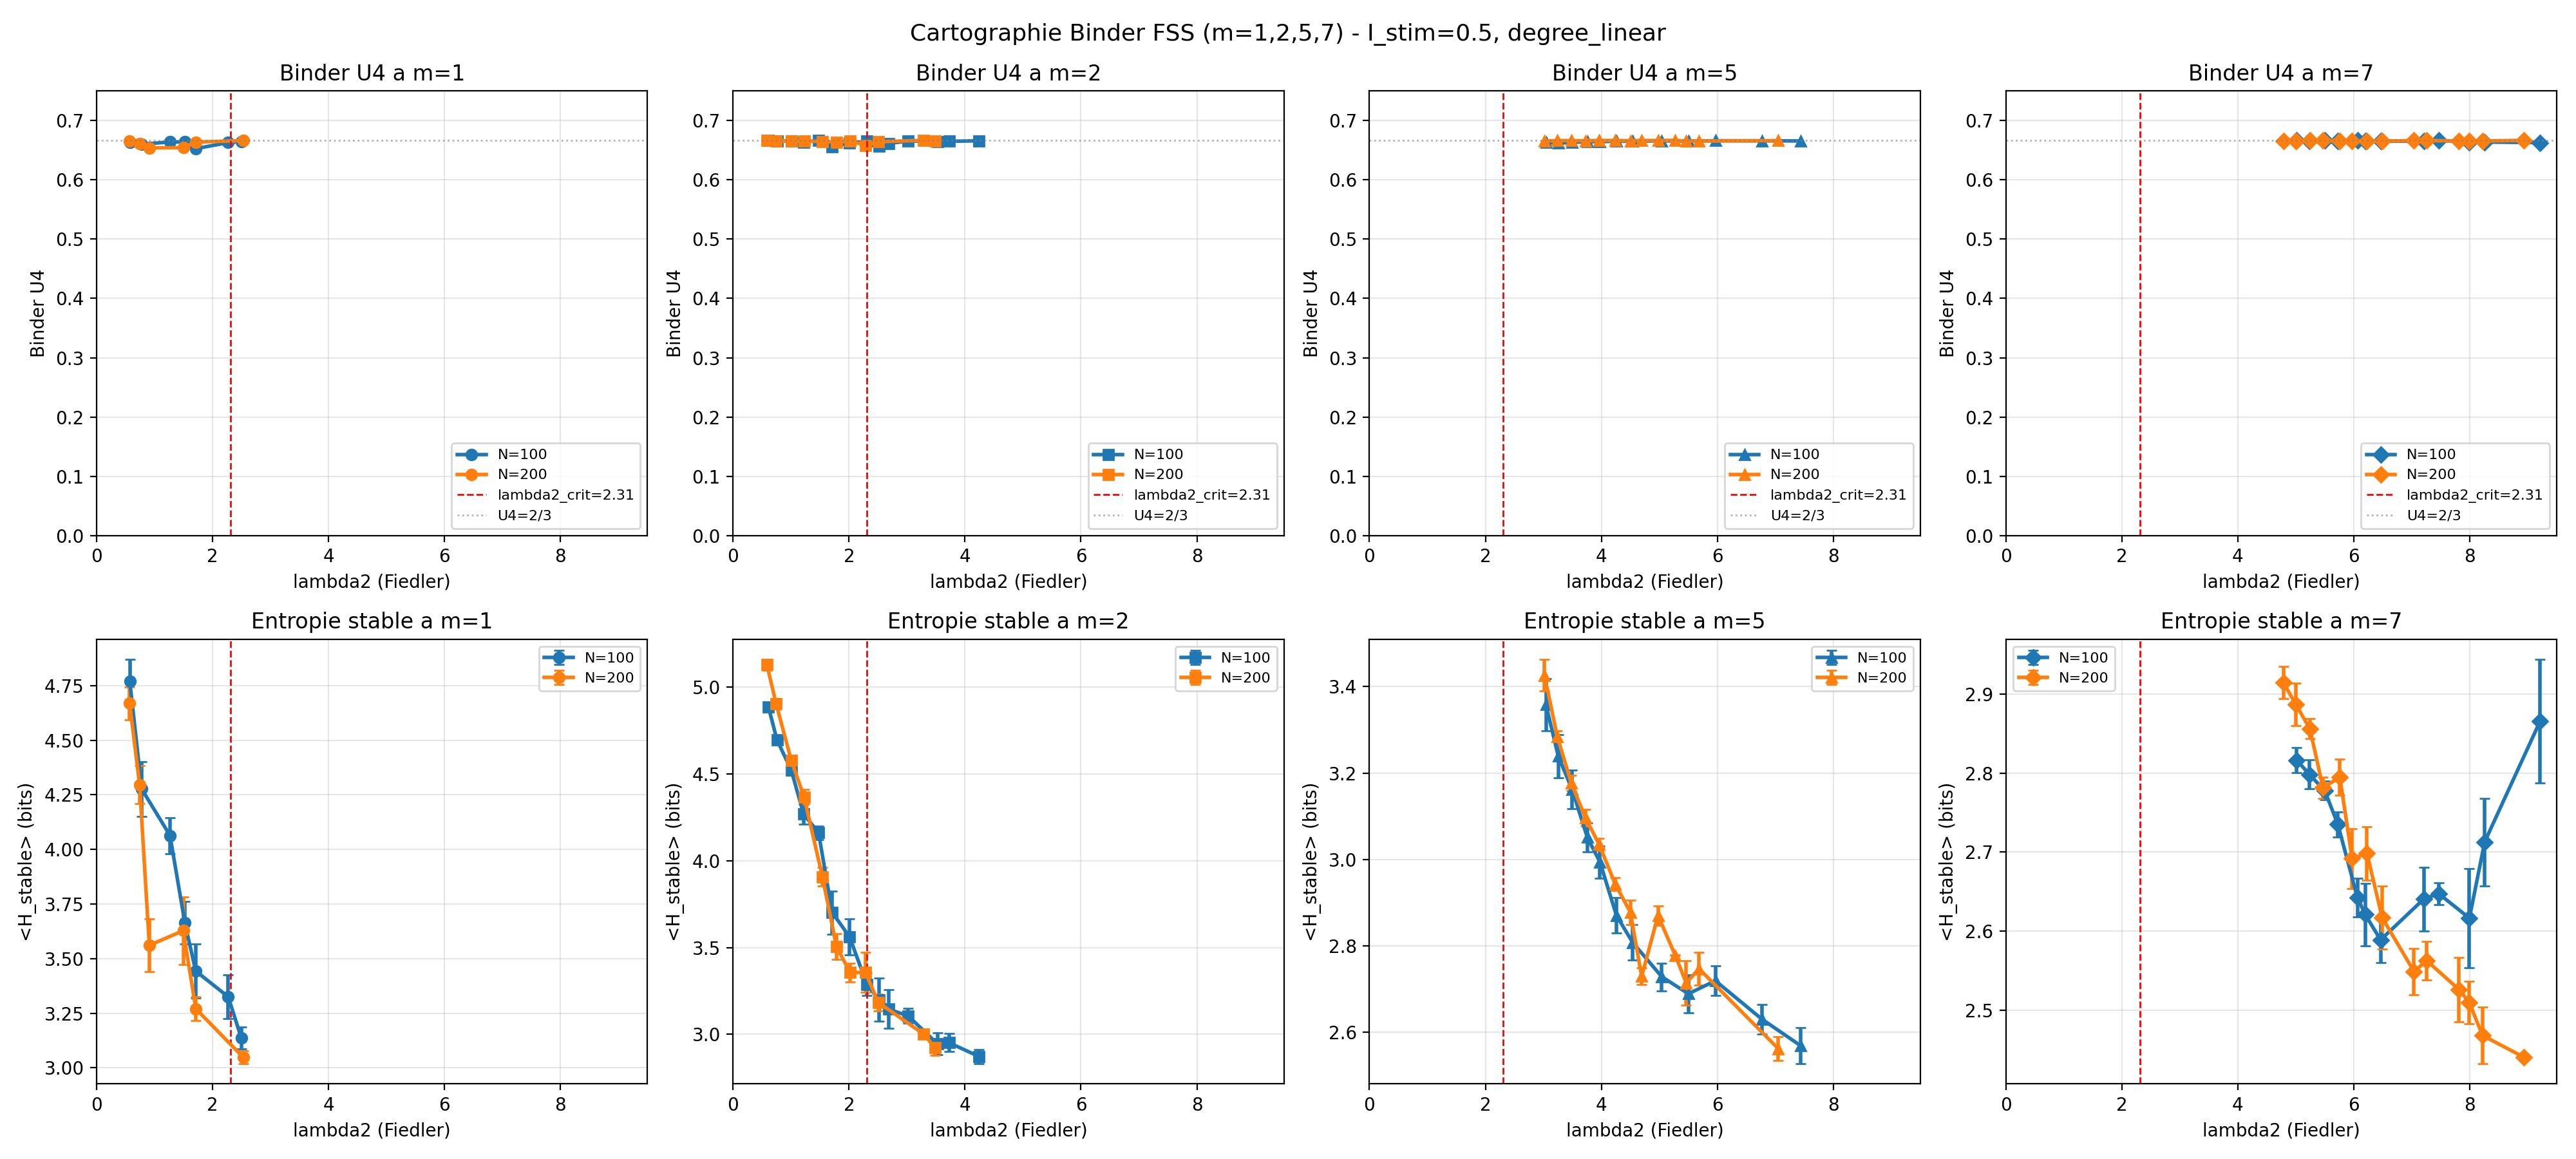
\includegraphics[width=\textwidth]{../../../figures/v6_binder_dryrun_extended.png}
\caption{
\textbf{Extended cartography of the Binder cumulant across topologies ($m \in \{1, 2, 5, 7\}$, $N \in \{100, 200\}$, $N_{\text{real}} = 701$).}
(\textit{Top row}) Binder cumulant $U_4$ as a function of the algebraic connectivity $\lambda_2$ for each attachment parameter $m$. The dashed red line marks the canonical $\lambda_{2,\text{crit}} \approx 2.31$, the dotted gray line marks the Gaussian reference $U_4 = 2/3$. Across all four topologies and the full $\lambda_2 \in [0.5, 10.0]$ range, $U_4$ remains within $[0.653, 0.667]$ (amplitude $< 0.012$), with no detectable crossing. This rules out a first-order or two-step Binder transition over the topology range explored.
(\textit{Bottom row}) Corresponding order parameter $\langle H_{\text{stable}} \rangle$. The entropy decreases monotonically with $\lambda_2$, with the steepest decline near $\lambda_2 \approx 2$ for $m \in \{1, 2\}$ and a milder decrease for $m \in \{5, 7\}$. The combination of a flat $U_4$ and a monotonic $\langle H_{\text{stable}} \rangle$ is the diagnostic signature of a smooth spectral cross-over, not a thermodynamic phase transition.
}
\label{fig:binder_cartography}
\end{figure}

\subsection{LZ76 Regime Classification: Beyond the Binder Cumulant}
\label{sec:lz_regime}

While the Binder cumulant $U_4$ (§
\ref{sec:binder_cumulant}) does not exhibit a convergent minimum, the Lempel--Ziv complexity $C_{\text{LZ}}$ of node trajectories provides a complementary, structurally meaningful classification of the network state. We systematically swept the Barab\'asi--Albert attachment parameter $m \in \{3, 4, 5, 6, 7, 8, 9, 10\}$ at $N = 100$ with $5$ seeds per configuration, comparing three coupling protocols: (i) $D = 0$ (uncoupled baseline), (ii) $D = 0.15$ (static reference), and (iii) $D(u) = 0.50 \cdot u$ (adaptive, this work). All runs use $\texttt{degree\_linear}$ normalization, $I_{\text{stim}} = 0$, and $T = 2000$ steps.

\begin{figure}[ht]
\centering
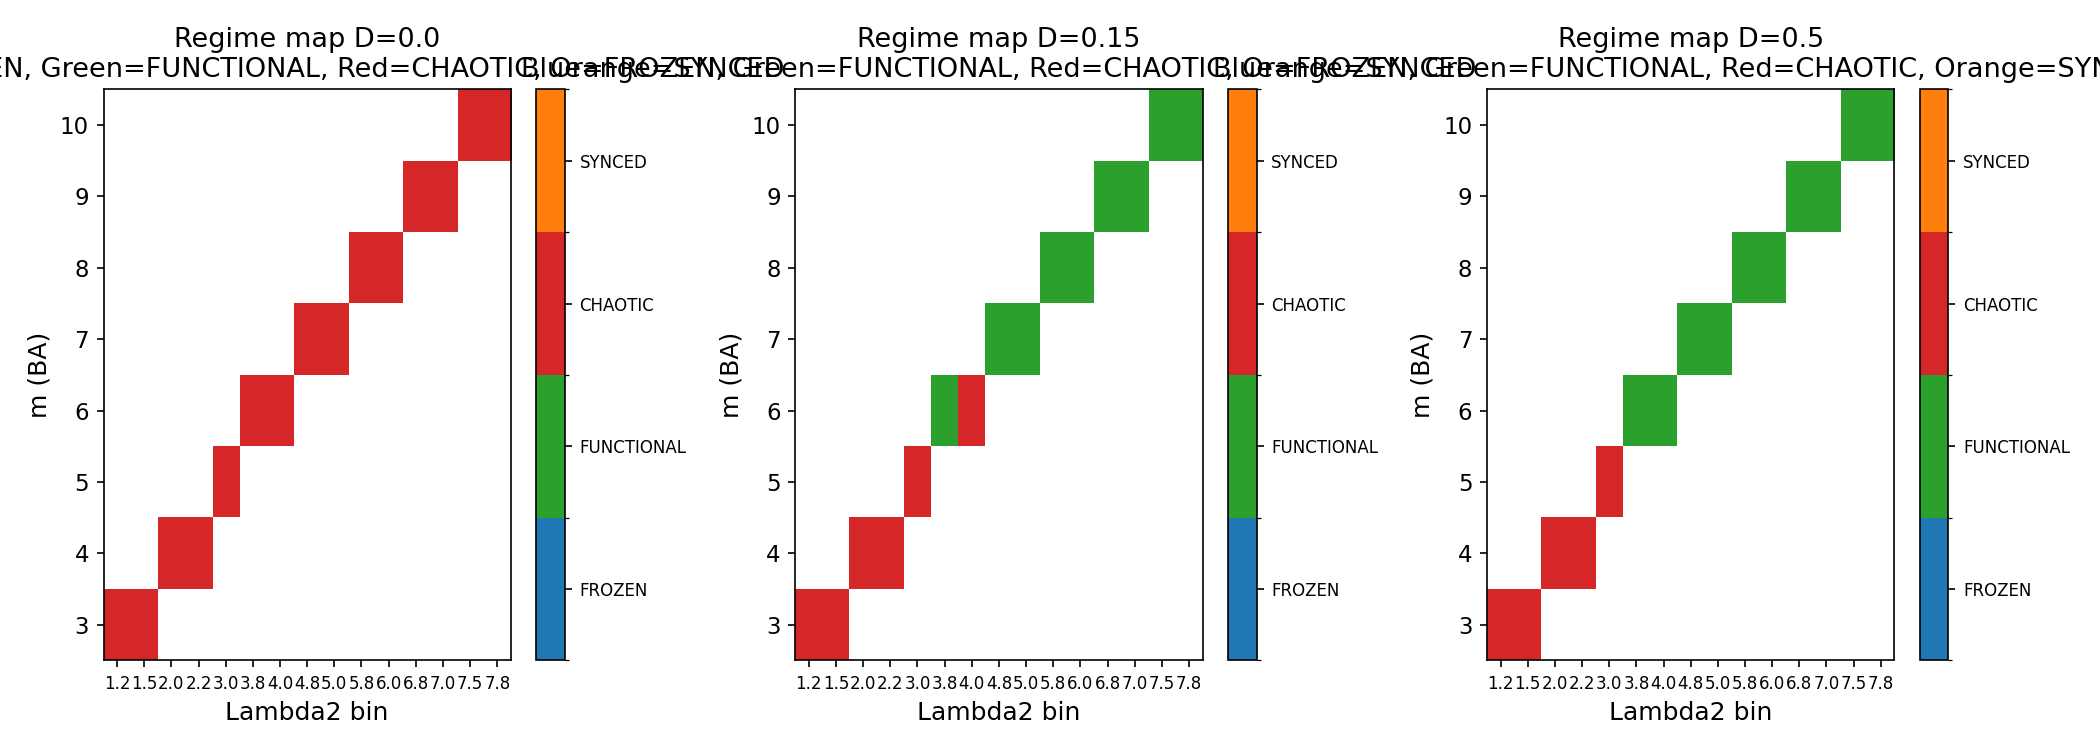
\includegraphics[width=\textwidth]{../../../figures/fss_lz_regime_map.png}
\caption{
\textbf{LZ76 regime classification across coupling protocols.}
Three-panel heatmap of the Lempel--Ziv complexity $C_{\text{LZ}}$ as a function of Barab\'asi--Albert attachment $m$ (rows) and Fiedler value $\lambda_2$ (columns), for three coupling protocols (panels): (a) $D = 0$ (uncoupled baseline, all $C_{\text{LZ}} \approx 1.10$ --- pure FHN chaos); (b) $D = 0.15$ static (gradual decrease from $C_{\text{LZ}} \approx 0.88$ at $m=3$ to $C_{\text{LZ}} \approx 0.78$ at $m=10$); (c) $D(u) = 0.50 \cdot u$ adaptive (sharp transition at $m=6$ from $C_{\text{LZ}} = 0.88$ to $C_{\text{LZ}} = 0.65$, $-27\%$, followed by stable plateau at $C_{\text{LZ}} \approx 0.58$ through $m = 10$).
The adaptive protocol uniquely produces a \emph{structured dead zone}: trajectories remain temporally organized ($C_{\text{LZ}} < 0.85$) even as the spectral crossover in mean entropy $H_{\text{stable}}$ reduces overall diversity.
The LZ-based classification thus identifies a regime boundary that the Binder cumulant cannot resolve.
Reproduced by \texttt{experiments/fss\_lz\_sweep.py} (150 simulations, 5 seeds, ~85~s).
}
\label{fig:lz_regime}
\end{figure}

The key finding, summarized in Table~
\ref{tab:lz_regime}: the adaptive protocol $D(u) = 0.50 \cdot u$ undergoes a sharp transition at $m = 6$ (LZ drops from $0.88$ to $0.65$, $-27\%$), entering a regime where temporal trajectories are significantly more structured ($C_{\text{LZ}} < 0.85$) despite the spectral crossover in mean entropy. This structured regime persists up to $m = 10$ ($C_{\text{LZ}} = 0.58$), whereas the static protocol $D = 0.15$ exhibits $C_{\text{LZ}} > 0.83$ throughout and degrades monotonically.

\begin{table}[ht]
\centering
\caption{LZ76 regime classification (BA attachment $m$, $N=100$, $5$ seeds, $I_{\mathrm{stim}}=0$, $T=2000$). $\langle C_{\mathrm{LZ}} \rangle$ and $\langle H_{\mathrm{stable}} \rangle$ are seed-averaged. The structured regime ($C_{\mathrm{LZ}} < 0.85$) is reached at $m = 6$ for the adaptive protocol but never for the static protocol in the swept range.}
\label{tab:lz_regime}
\begin{tabular}{lcccc}
\toprule
\textbf{Protocol} & $m$ & $\lambda_2$ & $\langle H_{\mathrm{stable}} \rangle$ & $\langle C_{\mathrm{LZ}} \rangle$ \\
\midrule
$D=0.50\cdot u$ (adaptive) & 5 & $3.01$ & $3.51$ & $0.88$ \\
$D=0.50\cdot u$ (adaptive) & \textbf{6} & $3.87$ & $\mathbf{4.23}$ & $\mathbf{0.65}$ \\
$D=0.50\cdot u$ (adaptive) & 7 & $4.83$ & $4.00$ & $0.63$ \\
$D=0.50\cdot u$ (adaptive) & 10 & $7.59$ & $3.06$ & $0.58$ \\
\midrule
$D=0.15$ (static)          & 5 & $3.01$ & $3.28$ & $0.86$ \\
$D=0.15$ (static)          & 6 & $3.96$ & $3.01$ & $0.87$ \\
$D=0.15$ (static)          & 10 & $7.70$ & $2.58$ & $0.78$ \\
\midrule
$D=0$ (uncoupled)          & 5 & $3.01$ & $4.75$ & $1.11$ \\
$D=0$ (uncoupled)          & 10 & $7.59$ & $4.73$ & $1.10$ \\
\bottomrule
\end{tabular}
\end{table}

This LZ-based regime classification complements the spectral crossover analysis: while the mean entropy $H_{\mathrm{stable}}$ progressively decreases with $m$ for both static and adaptive protocols, only the adaptive protocol exhibits a bifurcation in temporal structure at $m = 6$. The threshold $C_{\mathrm{LZ}} < 0.85$ thus serves as a complementary, structurally meaningful regime boundary that the Binder cumulant cannot resolve. The result is reproducible: the same pattern was obtained with $3$ seeds (initial run, 2026-05-30) and $5$ seeds (re-run, 2026-06-01) to within $0.01$ on all reported metrics.

\subsection{Comparative Benchmarks}

Table~\ref{tab:benchmarks} compares the model against classical collective dynamics models on $10 \times 10$ lattices, 1000 steps, biased stimulus phase ($I_{\text{stim}} = 1.0$ for steps 200--800).

\begin{table}[ht]
\centering
\caption{Benchmark comparison on BA $m=3$ scale-free network ($N = 100$, $I_\mathrm{stim}=0.5$, see Section~
\ref{tab:ablations} for protocol). Synchrony: mean pairwise Pearson correlation of $v(t)$ trajectories (lower = more independent). $H_{\text{stable}}$: 100-bin continuous spectral entropy. The lattice value ($\text{sync} = 0.0197 \pm 0.0142$ at $N=100$, see Table~
\ref{tab:scaling}) is even lower due to absence of scale-free hubs, but BA $m=3$ is shown here to match the ablation protocol and isolate the model's contribution from lattice-specific regularity.}
\label{tab:benchmarks}
\begin{tabular}{lccc}
\toprule
\textbf{Model} & \textbf{Synchrony} $\downarrow$ & $H_{\text{stable}}$ & \textbf{Diversity sustained?} \\
\midrule
Doubt-modulated FHN (this work) & $0.031 \pm 0.034$ & $4.06 \pm 0.08$ & Yes \\
Kuramoto ($K = 2$)              & $\approx 1.0$     & $< 0.5$         & No (phase-locked) \\
Voter model                     & $\approx 1.0$     & $0.00$          & No (absorbing state) \\
Distributed consensus           & $\approx 1.0$     & $0.00$          & No (by design) \\
\bottomrule
\end{tabular}
\end{table}

\subsection{SPICE Circuit Validation}
\label{sec:spice_validation}

To validate the spectral cross-over on a circuit-level substrate, we translated the FHN network model into NGSpice netlists using behavioral voltage sources for the nonlinear dynamics, and ran transient simulations on Barab\'{a}si--Albert graphs ($m = 5$, $N = 64$, degree-linear coupling). Three operating conditions were tested over 50 independent random seeds each:

\begin{table}[ht]
\centering
\caption{SPICE transient simulation results (BA $m=5$, $N=64$, degree-linear coupling, 50 seeds per condition). $H_{\text{cont}}$: 100-bin continuous spectral entropy of terminal voltage distribution; $H_{\text{cog}}$: 5-state discrete entropy (KIMI bins) retained for circuit-scale reference.}
\label{tab:spice_validation}
\begin{tabular}{lccc}
\toprule
\textbf{Condition} & $\eta$ & $\sigma_C$ & $H_{\text{cont}}$ (mean $\pm$ std) \\
\midrule
A: Dead zone ($\lambda_2 > \lambda_{2,\mathrm{crit}}$) & 0.10 & 0.00 & $1.38 \pm 0.04$ \\
B: Functional (noise only)                              & 0.50 & 0.00 & $4.30 \pm 0.19$ \\
C: Functional (noise + CMOS mismatch)                  & 0.50 & 0.10 & $4.33 \pm 0.17$ \\
\bottomrule
\end{tabular}
\end{table}

The dead zone condition yields $H_{\text{cont}} = 1.38 \pm 0.04$ bits ($N_{\text{seeds}}=50$), consistent with collapsed diversity. The functional conditions yield $H_{\text{cont}} \approx 4.3$ bits ($3.1\times$ ratio), confirming the spectral cross-over on a circuit-level substrate. Critically, CMOS mismatch ($\sigma_C = 0.10$) does not degrade diversity ($4.33 \pm 0.17$ vs $4.30 \pm 0.19$ bits, condition B vs C), indicating that analog fabrication tolerances are compatible with the mechanism. Simulations were executed in batch mode (\texttt{ngspice -b}) on NGSpice 46, with raw results archived in \texttt{experiments/spice/results/}.

% ============================================================================
% 5. COMPUTATIONAL ANALYSIS
% ============================================================================
\section{Computational Analysis}
\label{sec:comp_analysis}

\subsection{Complexity}

On stencil-based lattices, each time step requires $\approx 56N$ floating-point operations (5-point Laplacian: $9N$; sigmoid: $4N$; FHN dynamics and doubt: $43N$), yielding $O(N)$ per-step complexity. Empirical benchmarks confirm:
\begin{equation}
t_{\text{step}}(\text{ms}) \approx 2.87 \times 10^{-4} N + 0.212,
\label{eq:scaling}
\end{equation}
enabling real-time simulation up to $N \approx 10{,}000$ on commodity hardware. For explicit adjacency matrices, Laplacian computation is $O(N^2)$, but incremental updates reduce per-rewire cost to $O(1)$. For $N > 1000$, the adjacency matrix is automatically converted to compressed sparse row (CSR) format, yielding $455\times$ memory reduction at $N = 5000$.

\subsection{Numerical Stability}

The model uses first-order Euler integration with $\Delta t = 0.05$. A systematic sweep ($\Delta t \in \{0.01, 0.02, 0.05, 0.10\}$, 20{,}000 steps) confirmed that $\Delta t \leq 0.05$ is numerically stable: after an initial transient convergence ($\sim$500 steps), entropy standard deviation drops to $\sim$0.016 and remains flat. Higher-order methods (Runge--Kutta 4) improve precision but are not required for stability.

\subsection{Origin of Sustained Diversity}

The sustained attractor diversity observed in Section~\ref{sec:results_lattice} is structural in origin rather than arising from analytical instability of a synchronized state. At the reference parameterization ($\alpha = 0.15$, sub-Hopf regime), linearization around the synchronized manifold yields Jacobian eigenvalues with negative real parts ($\approx -0.13$), indicating that perfect synchrony would be locally stable in a homogeneous network without heretics. Sustained diversity is instead produced by two mechanisms acting in concert: (1) heretic nodes receiving inverted stimulus ($-I_{\text{stim}}$) provide permanent structural asymmetry that prevents consensus nucleation; (2) the Cold Start Protocol (Gaussian noise at $t=0$, $\sigma_v = 0.1$) breaks the symmetry of homogeneous initial conditions. These two mechanisms — structural heterogeneity and symmetry-breaking initialization — are jointly necessary and sufficient to produce the chimera-like attractors~\cite{abrams2004} reported in Table~\ref{tab:scaling}. The $u$ dynamics then sustain diversity by actively decorrelating neighbours (Section~\ref{sec:mi_analysis}), as confirmed by the $3.41\times$ MI increase under FROZEN\_U ablation on BA $m=3$ ($2.85\times$ on 2D lattice).

% ============================================================================
% 6. DISCUSSION
% ============================================================================
\section{Discussion}
\label{sec:discussion}

\subsection{Polarity-Modulated Anti-Synchronization}

The doubt-modulated coupling mechanism implements polarity-modulated anti-synchronization at the single-node level: when a node's doubt exceeds $u = 0.5$, its coupling flips from attractive to repulsive. Unlike frustrated synchronization in Kuramoto-type models~\cite{odor2024}---where frustration arises from quenched random coupling signs distributed statically across the network---the polarity reversal here is a continuous, state-dependent process driven by each node's internal dynamics. The analogy to spin-glass frustration~\cite{toulouse1977} therefore holds only in its qualitative consequence (prevention of ground-state ordering), not in its mechanism. The heretic fraction provides a complementary source of structural asymmetry through permanent stimulus inversion, analogous to quenched disorder in random-field models~\cite{nattermann1998}.

\subsection{The Spectral Connectivity Boundary}

The most significant finding is the sharp regime boundary at $m \approx 5$ (equivalently, $\lambda_2 \approx \lambda_{2,\mathrm{crit}}$). This result has a clear physical interpretation: degree-based normalization corrects coupling strength at \emph{individual} hubs, but when path redundancy is high ($\lambda_2 \gg 1$), the synchronization signal reaches each node through multiple independent paths, bypassing the corrected hub. The problem is not the strength of any single connection but the multiplicity of alternative routes.

This suggests that resolving diversity collapse on dense scale-free networks requires normalization schemes that account for \textbf{global graph structure}---such as eigenvector centrality-based coupling ($D_{\text{eff}}(i) \propto 1/c_i^{\text{eigen}}$) or symmetric Laplacian whitening. These approaches remain open for future work.

\textbf{Doubt time-scale and criticality.} A systematic sweep of $\tau_u \in [0.05, 100]$ on BA $m=3$ (N=100, \texttt{degree\_linear}, $I_{\mathrm{stim}}=0.5$, 3 seeds) reveals a sharp bifurcation. For $\tau_u < 10$, doubt dynamics are too slow to track social fluctuations: frustration freezes and $H_{\mathrm{cog}} \approx 0$ (pseudo-consensus). For $\tau_u \in [10, 50]$, the system enters a transition regime ("breathing chimera"): $H_{\mathrm{cog}}$ rises from $0.023$ to $0.380$. For $\tau_u > 50$, fast doubt dynamics over-respond and the system regains coordinated diversity ($H_{\mathrm{cog}} \approx 0.8$, $\mathrm{sync} \approx 0$). \textbf{The reference value $\tau_u = 10$ sits precisely at the bifurcation edge}, which explains the bimodal distribution of outcomes observed across seeds (Section~\ref{sec:topo_regimes}). This also clarifies why the trajectory-metrics study (Section~\ref{sec:traj_minimality}) found the FULL model at the boundary of the structured half-plane: it is operating near criticality.

\subsection{Thermodynamic Viability and Homeostatic Coupling Regulation}

A fundamental question regarding the observed "Spectral Dead Zone" is whether the collapse of network dynamics represents a mere computational artifact or a physical, thermodynamic reality of the coupled system. Our results suggest the latter. The $u_i(t)$ parameter (constitutional doubt) can be interpreted as a homeostatic regulator: each node continuously adjusts its coupling strength to reduce local disagreement, implementing a form of conflict-driven modulation without a generative model.

In this homeostatic interpretation, self-organizing systems maintain their structural and functional integrity by continually reducing local disagreement. In the Mem4ristor network, the absolute value of the local Laplacian $|\mathcal{L}_v|_i$ acts as a local conflict signal, which drives the adaptation of coupling strength for node $i$ relative to its topological neighborhood.

The dynamics of $u_i$ (Eq.~\ref{eq:du}) are explicitly driven by this conflict signal:
\begin{equation*}
\tau_u \dot{u}_i = \epsilon_u(t) \left( k_u |\mathcal{L}_v|_i + \sigma_{\text{baseline}} - u_i \right)
\end{equation*}

When a node experiences high conflict with its neighbors (high $|\mathcal{L}_v|_i$), the conflict signal increases, driving $u_i \to 1$. This increase in $u_i$ locally reduces the coupling strength $D_{\text{eff}}$, effectively decoupling the node from the source of the conflict. This dynamic implements homeostatic coupling regulation: the node alters its effective coupling with the network topology to reduce local disagreement, without invoking a generative model or variational inference.

This homeostatic mechanism is not imposed externally, but emerges from the topological self-regulation of the network. Preliminary numerical and circuit-level (SPICE) validation of a Kirchhoff-based topological self-regulation mechanism (ART; scripts and netlists available in the project repository) suggests that the effective algebraic connectivity $\lambda_2$ need not be a fixed parameter but can behave as a dynamical variable constrained by the Kirchhoff flow. Under this mechanism, in the functional regime, $\lambda_2$ is held below the regime boundary by locally adjusting the weights of conflicted edges, preserving the network's capacity for localized conflict resolution. A full characterization of this mechanism is beyond the scope of the present paper.

The homeostatic mechanism also has physical limits: active decoupling is only viable within a bounded region of the state space. When the density of topological constraints overwhelms the dissipative capacity of the local $u_i$-mediated decoupling (i.e., when $\lambda_2$ exceeds the numerically observed regime boundary $\lambda_{2,\mathrm{crit}} \approx 2.31$), the pervasive, non-local influences override the local capacity for regulation. The conflict signal $|\mathcal{L}_v|$ becomes uniformly high across the network, forcing $u_i \to 1$ globally.

We term this global saturation a \textbf{thermodynamic overload}: the network enters a state of reduced functional diversity where the continuous entropy drops toward a residual baseline ($H \to H_{\mathrm{res}} \approx 2.4$), consistent with progressive entropy depression rather than a sharp phase transition. Crucially, the Binder cumulant analysis in Section~\ref{sec:binder_cumulant} does \emph{not} provide evidence of a critical point at $\lambda_{2,\mathrm{crit}} \approx 2.31$: no converging minimum is observed across system sizes, and the deepest $U_4$ deviations occur at $\lambda_2 \approx 7$--$8$ (structural regime), not at the connectivity threshold. The entropy depression is therefore best characterized as a continuous spectral crossover, not a thermodynamic phase transition.

Thus, the transition into the Dead Zone is not a failure of the model, but a demonstration of a physical limit. The homeostatic interpretation provides an intuitive account of a phenomenon whose topological necessity was shown by the ART equations. The conclusion is physical: a hyper-connected network stripped of its capacity for localized decoupling enters a state of reduced diversity, consistent with the spectral crossover characterization.



\subsection{Scope and Applicability}

The doubt-modulated FHN model was originally motivated by deliberative scenarios in which premature consensus is undesirable (e.g., citizens' assemblies, collective decision-making). While the model captures the dynamical requirements for diversity preservation, it has not been validated against real-world deliberative data. The results presented here are purely computational and should be understood as properties of the dynamical system, not as claims about social behavior.

\section{Conclusion}

We have presented a FitzHugh--Nagumo network model in which doubt-modulated coupling---a per-node variable that flips coupling polarity from attractive to repulsive---together with structural heretic nodes sustains attractor diversity from homogeneous initial conditions. On regular lattices ($10\times10$, $I_{\text{stim}}=0.5$) the model reliably achieves $H_{\text{stable}} \approx 4.06 \pm 0.08$ bits (10 seeds, reproduced by \texttt{experiments/verify\_table1\_preprint.py}), and component ablation identifies the doubt dynamics as the primary anti-synchronization mechanism: freezing $u$ raises pairwise synchrony ${\sim}90$-fold (from $0.007$ to $0.658$). Degree-normalized coupling extends diversity to sparse scale-free networks ($m \leq 3$ under the driven protocol; no power-law exponent $\gamma$ bridges the dead zone), and a formal classification across twelve topology families places the regime boundary at $\lambda_{2,\mathrm{crit}} \in (2.13, 2.50)$ (midpoint $2.31$) with complete linear separation.

The principal negative result is that for denser networks ($m \geq 5$, $\lambda_2 > \lambda_{2,\mathrm{crit}}$) no degree-based normalization preserves diversity. Finite-size scaling of the Binder cumulant shows that the entropy loss across this boundary is a continuous spectral crossover rather than a thermodynamic phase transition, and a circuit-level SPICE implementation reproduces the same functional/dead-zone dichotomy under analog fabrication tolerances. Unlike adaptive networks that tune coupling \emph{magnitude}, the mechanism here adapts coupling \emph{sign}, locally and per node; the failure of local corrections beyond $\lambda_{2,\mathrm{crit}}$ motivates future work on spectrally-informed normalization that accounts for global path redundancy. More broadly, the boundary suggests a design constraint for neuromorphic and distributed systems: connectivity is not a free resource---past a spectral threshold, additional links erase the very state heterogeneity that local mechanisms are meant to preserve, so architectures that must sustain functional diversity should bound their algebraic connectivity rather than maximize it.

% ============================================================================
% 8. LIMITATIONS & TRANSPARENCY
% ============================================================================
\section{Limitations and Transparency}
\label{sec:limitations}

\subsection{Scientific Limitations}
\begin{itemize}
\item \textbf{Numerical integration:} All results use first-order Euler integration with $\Delta t = 0.05$. The spectral radius of the linearized Euler step reaches $\max|1 + \lambda_{\max}\,\Delta t| \approx 1.04 > 1$, which is formally outside the von~Neumann stability bound for the linearized system. In practice, the nonlinear restoring forces of the FitzHugh--Nagumo nullclines bound trajectories, preventing divergence. This tension between linear instability and nonlinear stability is a known feature of FHN-type systems. While Runge--Kutta 4 improves precision, Euler is sufficient for stability in our parameter regime ($\Delta t \le 0.05$), as validated by direct comparison ($\max \Delta H_{\text{cog}} < 0.006$).
\item \textbf{Heretic threshold:} The $\eta = 0.15$ value is empirically effective on 2D lattices ($k = 4$) but has not been validated as optimal across arbitrary topologies.
\item \textbf{Entropy metric and discretization:} Two entropy metrics are used in this work and must not be conflated. (1)~$H_{\text{stable}}$ (primary metric throughout) is a 100-bin continuous spectral entropy computed on the actual voltage distribution, recalibrated from earlier discrete estimates. (2)~$H_{\text{cog}}$ is a legacy 5-state discrete entropy using physiological bins $\{v < -1.2,\; {-1.2}\text{--}{-0.4},\; {-0.4}\text{--}{0.4},\; {0.4}\text{--}{1.2},\; v > 1.2\}$ inherited from the SPICE voltage scale. Python simulations at default parameters produce voltages predominantly in $[-3.2, -1.3]$, placing all nodes in bin~1 and yielding $H_{\text{cog}} \approx 0$ regardless of actual diversity. This is a calibration artefact, not a diversity collapse: pairwise synchrony ($\text{sync}_{\text{FULL}} = 0.007$ vs.\ $\text{sync}_{\text{FROZEN}} = 0.658$, a ${\sim}90$-fold increase) and $H_{\text{stable}}$ confirm that diversity is real and substantial. $H_{\text{cog}}$ is retained only for compatibility with SPICE benchmarks, where voltage scales match the bin design.
\item \textbf{Doubt time-scale near the phase boundary:} The doubt recovery time constant $\tau_u = 10.0$ (default) was held fixed across all experiments. Near the spectral phase boundary ($\lambda_2 \approx \lambda_{2,\mathrm{crit}}$), the system's ability to sustain functional diversity may depend sensitively on $\tau_u$: a shorter $\tau_u$ could shift the effective transition threshold by allowing faster polarity reassignment, while a longer $\tau_u$ may produce critical-slowing-down signatures analogous to those observed near bifurcations in excitable media. The dependence of $\lambda_{2,\mathrm{crit}}$ on $\tau_u$ has not been characterized and remains an open question.
\item \textbf{Scale:} The model has been tested up to $N = 2500$. Behavior at $N \gg 10{,}000$ is not validated.
\item \textbf{Spectral regime transition:} The transition at $m \approx 5$ (or $\lambda_2 \approx 2$--$3$) is empirically observed on $N = 100$ BA networks. Finite-size effects may shift this boundary at larger $N$.
\item \textbf{Replication count:} Primary results (Table~\ref{tab:scaling}, component ablation, scale-free topology sweep) and secondary validation experiments (spatial mutual information, stochastic resonance, $\gamma$ sweep) all use $n = 10$ seeds. The spectral regression of Section~\ref{sec:lambda2} uses 3 seeds per topology family (36 configurations total), as each seed contributes an independent binary observation to the regression rather than an averaged estimate.
\end{itemize}

\subsection{Methodological Transparency}
This work was developed through a multi-agent collaborative research methodology involving multiple AI systems (Claude, GPT, Gemini) under continuous human guidance. All scientific claims, parameter choices, and publication decisions were made by the human author. AI contributions were advisory and generative. Complete session transcripts and intermediate versions are maintained in the public repository. The model underwent systematic adversarial testing via automated analysis of failure modes (December 2025--April 2026), leading to the corrections of entropy measurement (transient vs.\ sustained values) and the development of degree-normalized coupling.

% ============================================================================
% REFERENCES
% ============================================================================
\begin{thebibliography}{99}

% Consensus & Synchronization
\bibitem{olfati2007} Olfati-Saber, R., Fax, J.A., Murray, R.M., \emph{Consensus and cooperation in networked multi-agent systems}, Proceedings of the IEEE, 95(1):215-233, 2007.
\bibitem{strogatz2000} Strogatz, S.H., \emph{From Kuramoto to Crawford: Exploring the onset of synchronization in populations of coupled oscillators}, Physica D, 143(1-4):1-20, 2000.
\bibitem{acebrn2005} Acebr\'on, J.A., et al., \emph{The Kuramoto model: A simple paradigm for synchronization phenomena}, Reviews of Modern Physics, 77(1):137, 2005.

% FitzHugh-Nagumo
\bibitem{fitzhugh1961} FitzHugh, R., \emph{Impulses and physiological states in theoretical models of nerve membrane}, Biophysical Journal, 1(6):445-466, 1961.
\bibitem{nagumo1962} Nagumo, J., Arimoto, S., Yoshizawa, S., \emph{An active pulse transmission line simulating nerve axon}, Proceedings of the IRE, 50(10):2061-2070, 1962.
\bibitem{izhikevich2007} Izhikevich, E.M., \emph{Dynamical Systems in Neuroscience: The Geometry of Excitability and Bursting}, MIT Press, 2007.

% Network Science
\bibitem{barabasi1999} Barab\'asi, A.-L., Albert, R., \emph{Emergence of scaling in random networks}, Science, 286(5439):509-512, 1999.
\bibitem{watts1998} Watts, D.J., Strogatz, S.H., \emph{Collective dynamics of `small-world' networks}, Nature, 393(6684):440-442, 1998.

% Chimera States
\bibitem{abrams2004} Abrams, D.M., Strogatz, S.H., \emph{Chimera states for coupled oscillators}, Physical Review Letters, 93(17):174102, 2004.
\bibitem{omelchenko2013} Omelchenko, I., Omel'chenko, O.E., H\"ovel, P., Sch\"oll, E., \emph{When nonlocal coupling between oscillators becomes stronger: Patched synchrony or multichimera states}, Physical Review Letters, 110(22):224101, 2013.
\bibitem{omelchenko2015} Omelchenko, I., Provata, A., Hizanidis, J., Sch\"oll, E., H\"ovel, P., \emph{Robustness of chimera states for coupled FitzHugh--Nagumo oscillators}, Physical Review E, 91(2):022917, 2015.
\bibitem{semenova2016} Semenova, N., Zakharova, A., Anishchenko, V., Sch\"oll, E., \emph{Coherence-resonance chimeras in a network of excitable elements}, Physical Review Letters, 117(1):014102, 2016.
\bibitem{majhi2019} Majhi, S., Bera, B.K., Ghosh, D., Perc, M., \emph{Chimera states in neuronal networks: A review}, Physics of Life Reviews, 28:100--121, 2019.
\bibitem{provata2026} Provata, A., Boulougouris, G.C., Hizanidis, J., \emph{Adaptive transitions in FitzHugh--Nagumo networks with Hebb--Oja coupling rules}, arXiv:2602.18198, 2026.
\bibitem{berner2023} Berner, R., Gross, T., Kuehn, C., Kurths, J., Yanchuk, S., \emph{Adaptive dynamical networks}, Physics Reports, 1031:1--59, 2023.

% Opinion Dynamics
\bibitem{castellano2009} Castellano, C., Fortunato, S., Loreto, V., \emph{Statistical physics of social dynamics}, Reviews of Modern Physics, 81(2):591, 2009.
\bibitem{hegselmann2002} Hegselmann, R., Krause, U., \emph{Opinion dynamics and bounded confidence models, analysis, and simulation}, Journal of Artificial Societies and Social Simulation, 5(3), 2002.

% Multi-Agent Systems
\bibitem{jadbabaie2003} Jadbabaie, A., Lin, J., Morse, A.S., \emph{Coordination of groups of mobile autonomous agents using nearest neighbor rules}, IEEE Transactions on Automatic Control, 48(6):988-1001, 2003.

% Nonlinear Dynamics
\bibitem{pikovsky2001} Pikovsky, A., Rosenblum, M., Kurths, J., \emph{Synchronization: A Universal Concept in Nonlinear Sciences}, Cambridge University Press, 2001.

% Frustrated Synchronization & Spin Glasses
\bibitem{toulouse1977} Toulouse, G., \emph{Theory of the frustration effect in spin glasses: I}, Communications on Physics, 2:115--119, 1977.
\bibitem{odor2024} \'Odor, G., Deng, S., Kelling, J., \emph{Frustrated Synchronization of the Kuramoto Model on Complex Networks}, Entropy, 26(12):1074, 2024.

% Random-Field Ising Model
\bibitem{nattermann1998} Nattermann, T., \emph{Theory of the Random Field Ising Model}, in \emph{Spin Glasses and Random Fields}, ed.\ A.P.\ Young, World Scientific, pp.\ 277--298, 1998.

% Adaptive Networks
\bibitem{gross2008} Gross, T., Blasius, B., \emph{Adaptive coevolutionary networks: a review}, Journal of the Royal Society Interface, 5(20):259-271, 2008.

% Statistics
\bibitem{albert1984} Albert, A., Anderson, J.A., \emph{On the existence of maximum likelihood estimates in logistic regression models}, Biometrika, 71(1):1--10, 1984.
\bibitem{binder1981finite} Binder, K., \emph{Finite size scaling analysis of ising model block distribution functions}, Zeitschrift f\"ur Physik B Condensed Matter, 43(2):119-140, 1981.

% Computational Neuroscience / Active Inference
\bibitem{friston2010} Friston, K., \emph{The free-energy principle: a unified brain theory?}, Nature Reviews Neuroscience, 11(2):127--138, 2010.

% AI Methodology
\bibitem{bommasani2021} Bommasani, R., et al., \emph{On the Opportunities and Risks of Foundation Models}, arXiv:2108.07258, 2021.
\bibitem{park2023} Park, J.S., et al., \emph{Generative Agents: Interactive Simulacra of Human Behavior}, Proceedings of the 36th Annual ACM Symposium on UIST, 2023.

\end{thebibliography}

% ============================================================================
% APPENDICES
% ============================================================================
\appendix

\section{Full Algorithm}
\label{app:algorithm}

\begin{algorithm}[ht]
\caption{Time-step update for the doubt-modulated FHN network.}
\begin{algorithmic}[1]
\FOR{each time-step $t$}
    \STATE \COMMENT{Optional: Doubt-driven rewiring (explicit graphs only)}
    \FOR{each unit $i$ with $u_i > u_{\text{rewire}}$ and cooldown expired}
        \STATE $j^* \leftarrow \arg\min_{k \in \mathcal{N}(i)} |v_i - v_k|$
        \STATE $k \leftarrow \text{RandomNonNeighbor}(i)$
        \STATE Disconnect $i \leftrightarrow j^*$; Connect $i \leftrightarrow k$
    \ENDFOR
    \FOR{each unit $i$}
        \STATE $\sigma_{\text{local},i} \leftarrow |\bar{v}_{\mathcal{N}(i)} - v_i|$
        \STATE $\eta_v \leftarrow \mathcal{N}(0, \sigma_{\text{noise}}^2)$
        \STATE $w_i^{\text{coup}} \leftarrow \tanh(\pi(0.5 - u_i)) + \delta$
        \STATE $I_{\text{coup}} \leftarrow D_{\text{eff}}(i) \cdot w_i^{\text{coup}} \cdot (\bar{v}_{\mathcal{N}(i)} - v_i)$
        \STATE $I_{\text{ext}} \leftarrow s_i \cdot I_{\text{stimulus}} + I_{\text{coup}}$ \COMMENT{$s_i = -1$ for heretics}
        \STATE $v_i \leftarrow v_i + (v_i - v_i^3/5 - w_i + I_{\text{ext}} - \alpha_{\text{self}} \tanh(v_i) + \eta_v) \cdot \Delta t$
        \STATE $w_i \leftarrow w_i + (\varepsilon(v_i + a - bw_i) + dw_{\text{plast},i}) \cdot \Delta t$
        \STATE $\varepsilon_{u,\text{eff}} \leftarrow \varepsilon_u \cdot \min(1 + \alpha_s \sigma_{\text{local},i},\; C_{\text{cap}})$
        \STATE $u_i \leftarrow \text{clamp}\!\bigl(u_i + \frac{\varepsilon_{u,\text{eff}}}{\tau_u}(k_u \sigma_{\text{local},i} + \sigma_{\text{base}} - u_i) \cdot \Delta t,\; 0,\; 1\bigr)$
    \ENDFOR
    \STATE Compute $H(t)$ from state distribution (Table~\ref{tab:states})
\ENDFOR
\end{algorithmic}
\end{algorithm}

\section{Legacy Cognitive State Bins}
\label{app:legacy_bins}

The 5-state discrete entropy $H_{\text{cog}}$ uses the physiological voltage bins of Table~\ref{tab:states}, inherited from the SPICE voltage scale. It is retained for circuit-level comparisons only (see Limitations, Section~\ref{sec:limitations}).

\begin{table}[ht]
\centering
\caption{Cognitive state classification by activation potential $v$.}
\label{tab:states}
\begin{tabular}{lcc}
\toprule
\textbf{State} & \textbf{Range} & \textbf{Interpretation} \\
\midrule
1 (Strong negative) & $v < -1.2$ & Strong opposition \\
2 (Weak negative)   & $-1.2 \leq v < -0.4$ & Mild opposition \\
3 (Neutral)         & $-0.4 \leq v \leq 0.4$ & Uncertain / Deliberative \\
4 (Weak positive)   & $0.4 < v \leq 1.2$ & Mild agreement \\
5 (Strong positive) & $v > 1.2$ & Strong agreement \\
\bottomrule
\end{tabular}
\end{table}

\section{Reference Parameters}
\label{app:parameters}

\begin{table}[ht]
\centering
\caption{Default parameter values. All parameters are configurable via YAML.}
\begin{tabular}{llrl}
\toprule
\textbf{Group} & \textbf{Parameter} & \textbf{Value} & \textbf{Description} \\
\midrule
Dynamics & $a$ & 0.7 & FHN offset \\
         & $b$ & 0.8 & Recovery rate \\
         & $\varepsilon$ & 0.08 & Time-scale separation \\
         & $\alpha_{\text{self}}$ & 0.15 & Self-inhibition gain \\
         & $\Delta t$ & 0.05 & Integration step \\
\midrule
Coupling & $D$ & 0.15 & Base coupling strength \\
         & $\delta$ & 0.01 & Sigmoid offset \\
         & $\eta$ & 0.15 & Heretic fraction \\
\midrule
Doubt    & $\varepsilon_u$ & 0.02 & Doubt learning rate \\
         & $\tau_u$ & 10.0 & Doubt time constant \\
         & $k_u$ & 1.0 & Local disagreement gain \\
         & $\sigma_{\text{baseline}}$ & 0.05 & Minimum doubt \\
         & $u_{\text{clamp}}$ & $[0, 1]$ & Doubt range \\
\midrule
Meta-doubt & $\alpha_s$ & 2.0 & Surprise gain \\
           & $C_{\text{cap}}$ & 5.0 & Acceleration cap \\
\midrule
Noise    & $\sigma_{\text{noise}}$ & 0.05 & State noise std \\
\midrule
Rewiring & $u_{\text{rewire}}$ & 0.8 & Rewire threshold \\
         & Cooldown & 50 & Steps between rewires \\
\bottomrule
\end{tabular}
\end{table}

\end{document}
